\documentclass[12pt]{article}

\usepackage{caption} %interesting things with captions
\usepackage[margin=1.5in]{geometry} %mostly set margin of the report
\usepackage{tabulary} %text wrapping in tables
\usepackage{subcaption} %let me put multiple images into a single caption
\usepackage{textcomp} %let me use \textrangle{} to get '>'
\usepackage{hyperref} %links in ToC - should be mostly the last thing imported?

%images being embeded
\usepackage{graphicx}
\graphicspath{ {images/} }

%code highlighting
\usepackage{minted}
\setminted[c++]{frame=single,linenos=true,autogobble=true,numbersep=4pt,tabsize=4}
\setminted[bash]{frame=single,linenos=true,autogobble=true,numbersep=4pt,tabsize=4}
\setminted[xml]{frame=single,linenos=true,autogobble=true,numbersep=4pt,tabsize=4}

%fix a quote mark issue
\usepackage [english]{babel}
\usepackage [autostyle, english = american]{csquotes}
\MakeOuterQuote{"}

%page 129
\begin{document}
\pagenumbering{gobble}
\begin{titlepage}
	\centering
	{\Huge Iteration 2\par}
	\vspace{0.25in}
	{\Large Reddit Robot\par}
	\vspace{2in}
	{Alex Harper\par}
	\newpage
\end{titlepage}
\pagenumbering{roman}
\tableofcontents
\newpage
\pagenumbering{arabic}

\section{Use Cases}

Has the previous use cases with minor edits and some extras.

\hypertarget{Authenticate the User (session)}{
\subsection{Authenticate the User (session)}
}
\begin{itemize}
	\item No Refresh Token
	\begin{itemize}
		\item Prompt the user to visit the correct URL (includes scopes and program ID)
		\item Prompt the user to click "Allow" on the webpage
		\item Prompt the user to copy the URL they got redirected to back into the program
		\item Parse the URL for the temperary token
		\item Use the one-time-use token to get the session and refresh tokens
		\item Save the refresh token to disk
		\item Restart the session timeout timer
	\end{itemize}

	\item Has Refresh Token but not Session Token
	\begin{itemize}
		\item Use the refresh token to get a new session token
		\item Restart the session timeout timer
	\end{itemize}

	\item Has Session Token and Refresh Token
	\begin{itemize}
		\item If session timeout timer is past 3600 seconds, use \textit{Has Refresh Token but not Session Token}
	\end{itemize}
\end{itemize}

\hypertarget{Read Data (session)}{
\subsection{Read Data (session)}
}
\begin{itemize}
	\item \hyperlink{Authenticate the User (session)}{\textit{Authenticate the User}}
	\item Check that not too many requests have been made in the last time period
	\item Set the HTTP header
	\begin{itemize}
		\item Set the useragent string in the header
		\item Set the authorization string in the header
	\end{itemize}
	\item Make request
	\item Wait for reply to finish
	\item Get information from reply
	\begin{itemize}
		\item Get the \textit{X-Ratelimit-Remaining} number from the header (requests available left)
		\item Get the \textit{X-Ratelimit-Reset} number from the header (time until get more requests)
	\end{itemize}
	\item Return the body of the message
\end{itemize}

\subsection{Getting Subreddit Data}
\begin{itemize}
	\item Ask the \hyperlink{Read Data (session)}{session to retrieve data}
	\begin{itemize}
		\item url = "https://oauth.reddit.com/r/" + subreddit + "/about"
		\item Use the GET method
	\end{itemize}
	\item Make sure it is a JSON Object
	\item Make JSON object and begin the tedium of parsing it into the public variables
\end{itemize}

\subsection{Getting Subreddit Posts}
\begin{itemize}
	\item Ask the \hyperlink{Read Data (session)}{session to retrieve data}
	\begin{itemize}
		\item url = "https://oauth.reddit.com/r/" + subreddit
		\item Use the GET method
	\end{itemize}
	\item Make sure it is a JSON Object
	\item Make JSON object and begin the tedium of parsing it into a list
	\begin{itemize}
		\item Drill down the JSON stack to get the object for the array of posts
		\item Iterate through the array
		\item Make a new Post object for every index
		\item Add the new Post to the list
	\end{itemize}
	\item Return the list of Posts
\end{itemize}

\subsection{Getting Post Comments}
\begin{itemize}
	\item Ask the \hyperlink{Read Data (session)}{session to retrieve data}
	\begin{itemize}
		\item url = "https://oauth.reddit.com/" + permalink
		\item Use the GET method
	\end{itemize}
	\item Make sure it is a JSON Object
	\item Make JSON object and begin the tedium of parsing it into a list
	\begin{itemize}
		\item Drill down the JSON stack to get the object for the array of comments
		\item Iterate through the array
		\item Make a new Comment object for every index
		\item Add the new Comment to the list
	\end{itemize}
	\item Return the list of Comments
\end{itemize}

\subsection{Getting Current Account Data}
\begin{itemize}
	\item Ask the \hyperlink{Read Data (session)}{session to retrieve data}
	\begin{itemize}
		\item url = "https://oauth.reddit.com/r/api/v1/me"
		\item Use the GET method
	\end{itemize}
	\item Make sure it is a JSON Object
	\item Make JSON object and begin the tedium of parsing it into the public variables
\end{itemize}

\subsection{Other Cases I want to add later}
\begin{itemize}
	\item Getting a Certain Account's data
	\item Imgur read and write with their API
	\item Message content to parse for in my bot
\end{itemize}

\newpage
\section{Domain Diagram}
\begin{figure}[ht]
	\centering
	\caption{The Original Reddit Domain Diagram. It is mostly correct, but for accounts it is missing details.}
	\label{domain1}
	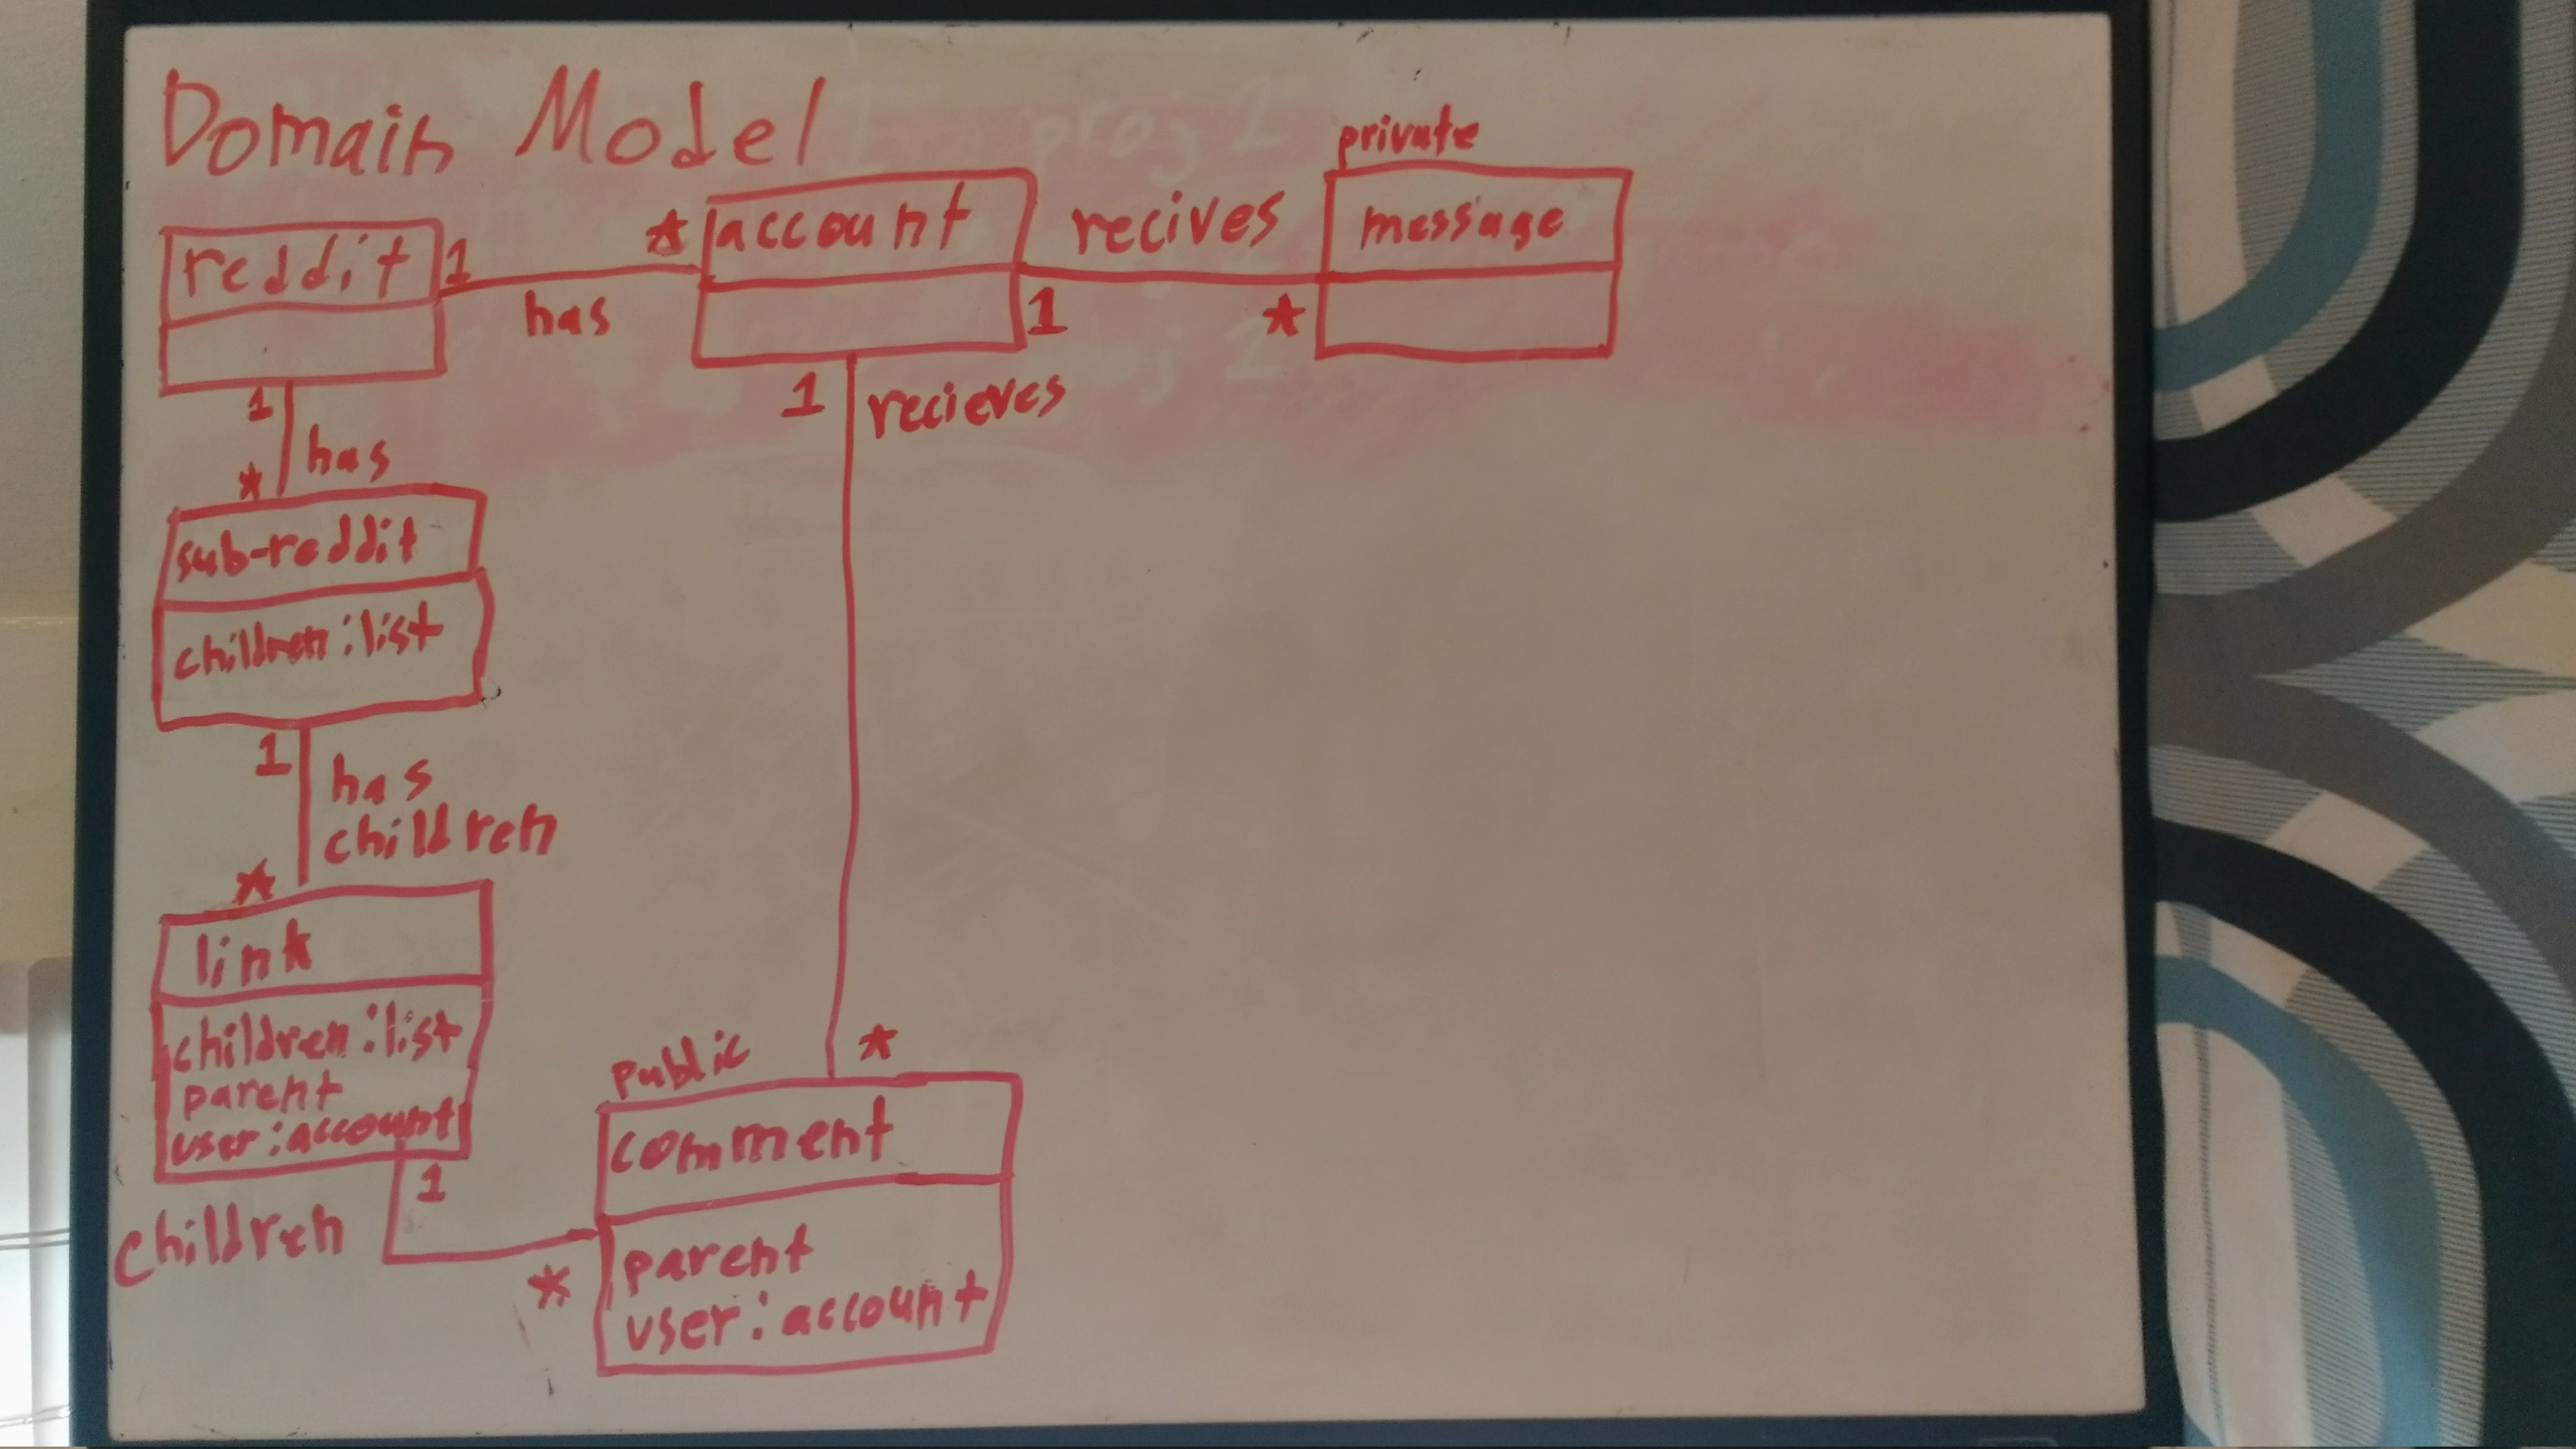
\includegraphics[width=0.8\textwidth]{domain1.jpg}
	\vspace{-10pt}
\end{figure}
\begin{figure}[ht]
	\centering
	\caption{The New Reddit Domain Diagram. This was made in the middle of the iteration when I had figured out all the parts.}
	\label{domain2}
	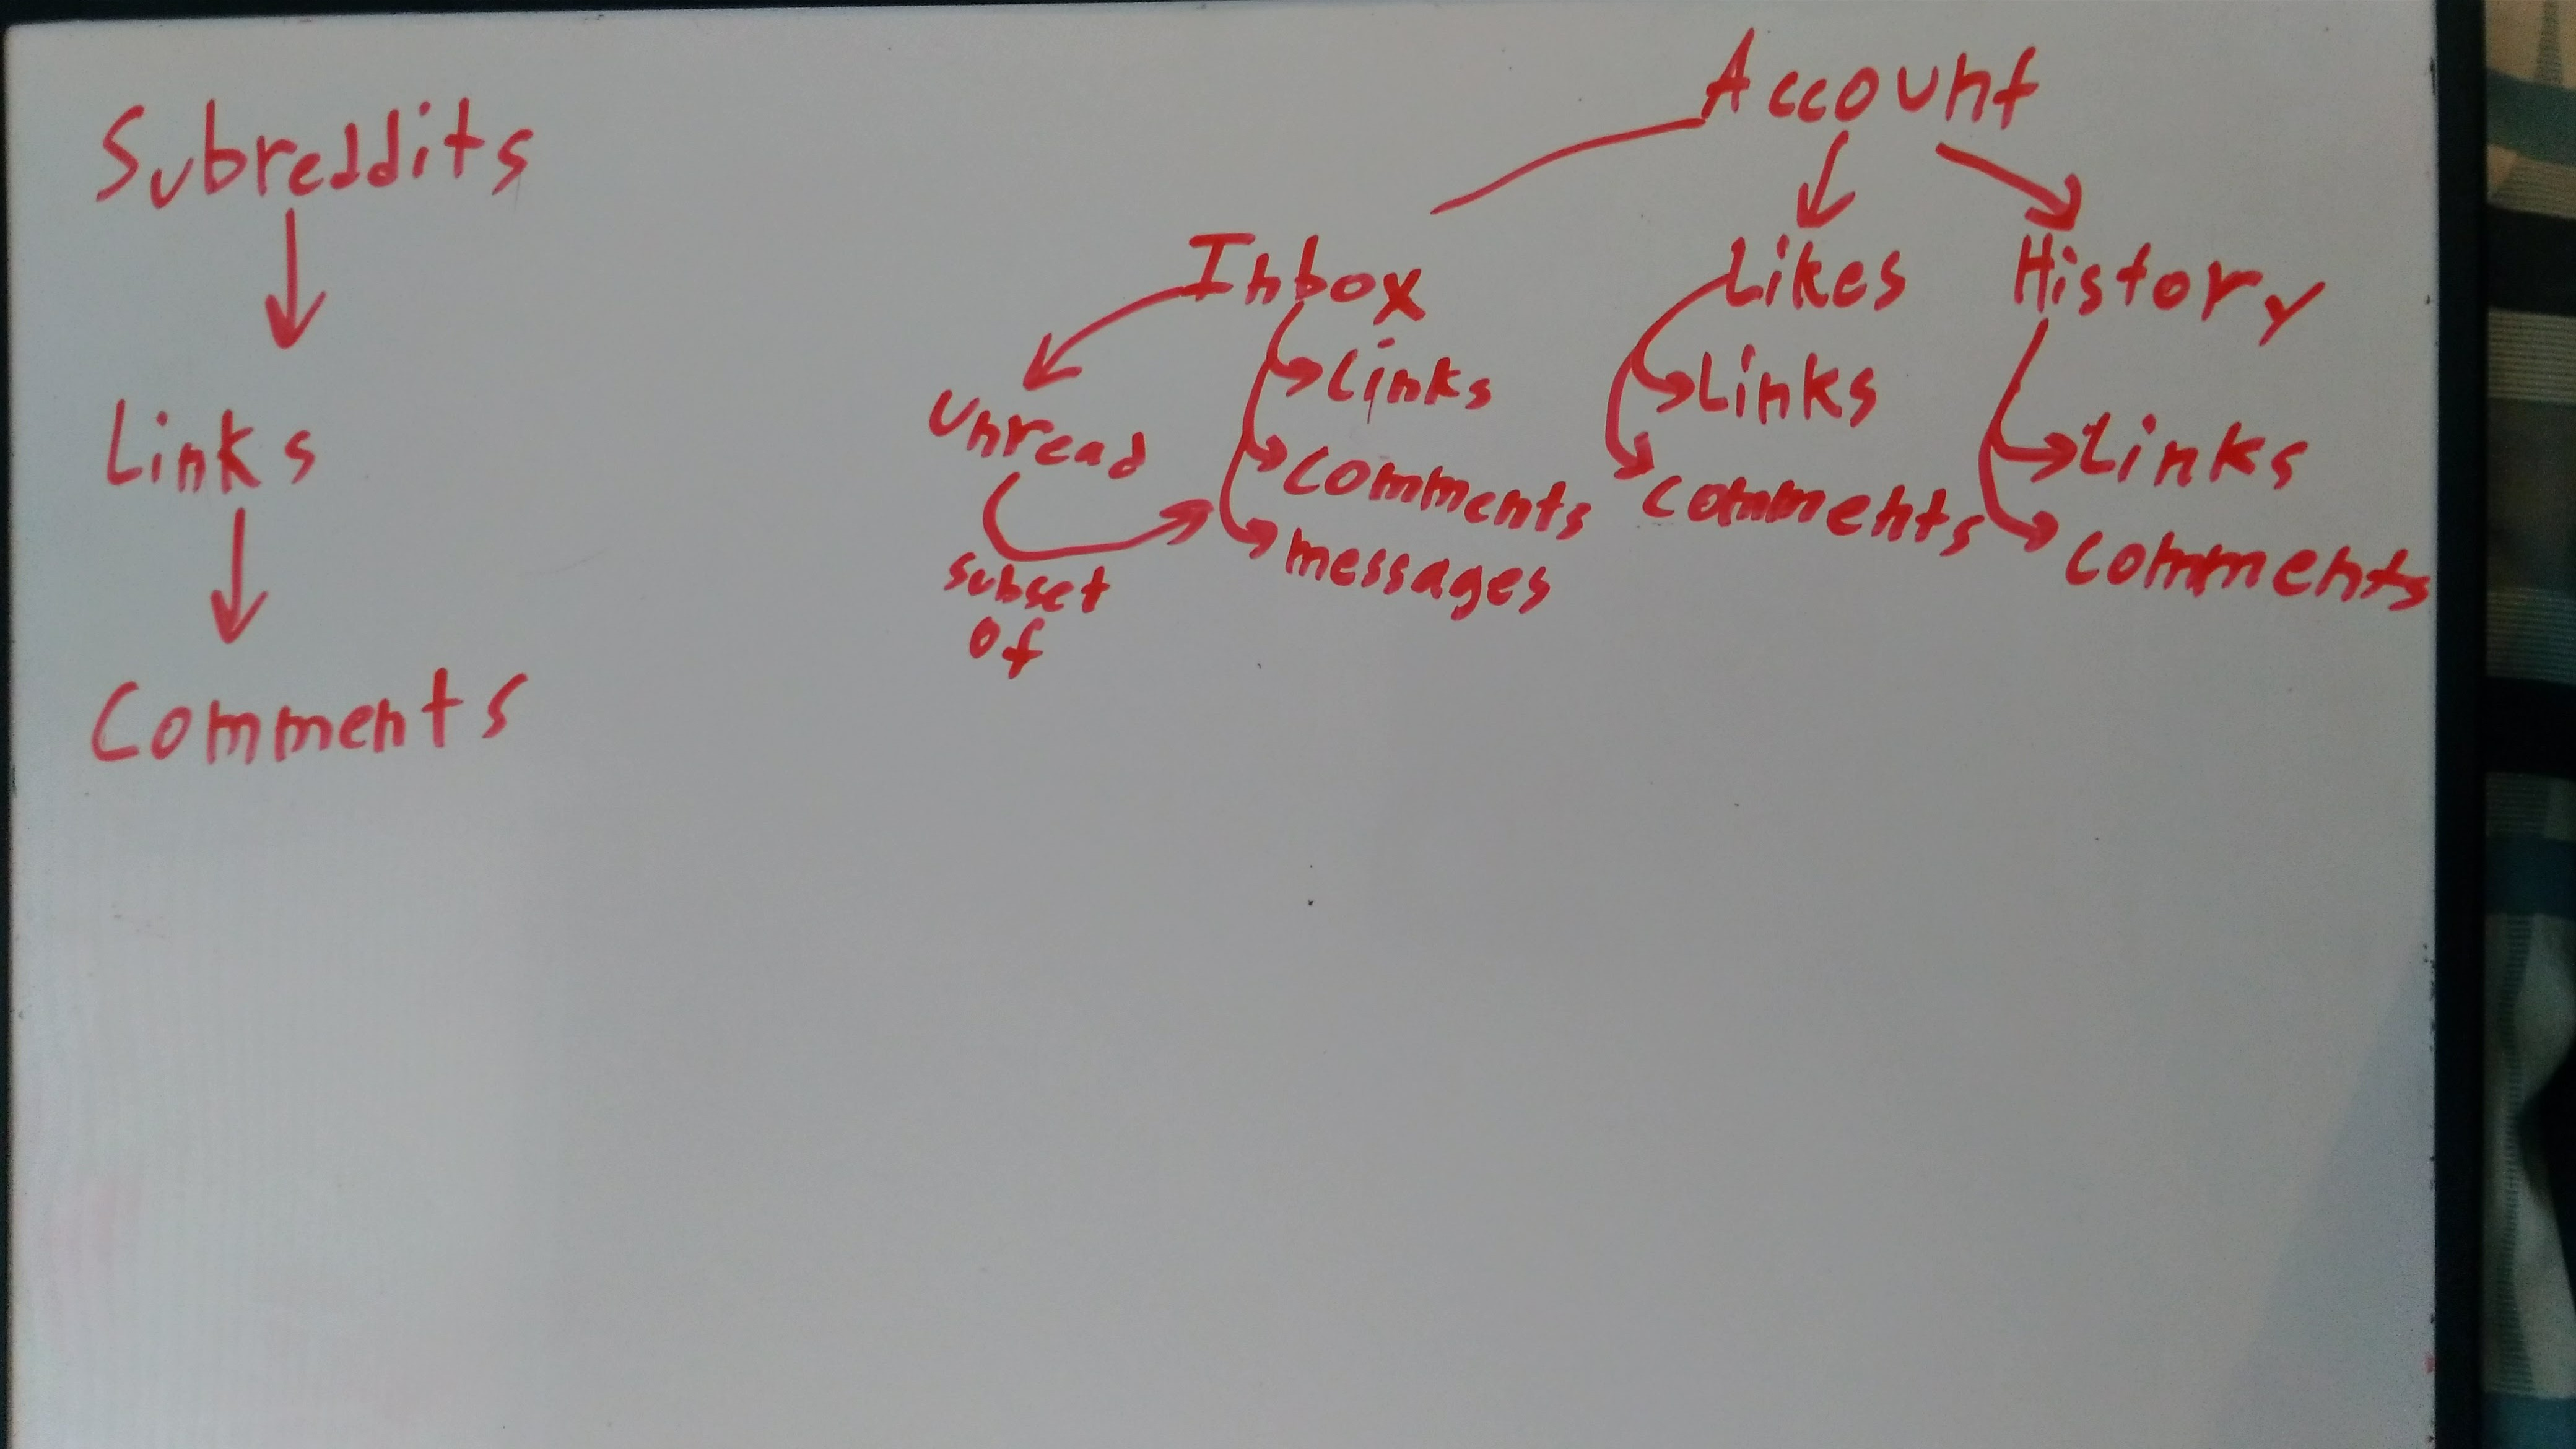
\includegraphics[width=0.8\textwidth]{domain2.jpg}
	\vspace{-10pt}
\end{figure}

\clearpage
\section{Reading Data}
\begin{figure}[ht]
	\centering
	\caption{Original Sequence Diagram Example for Getting Data. It was at a time when JSON was not really thought about, and simply that strings of some sort would come back.}
	\label{sequence1}
	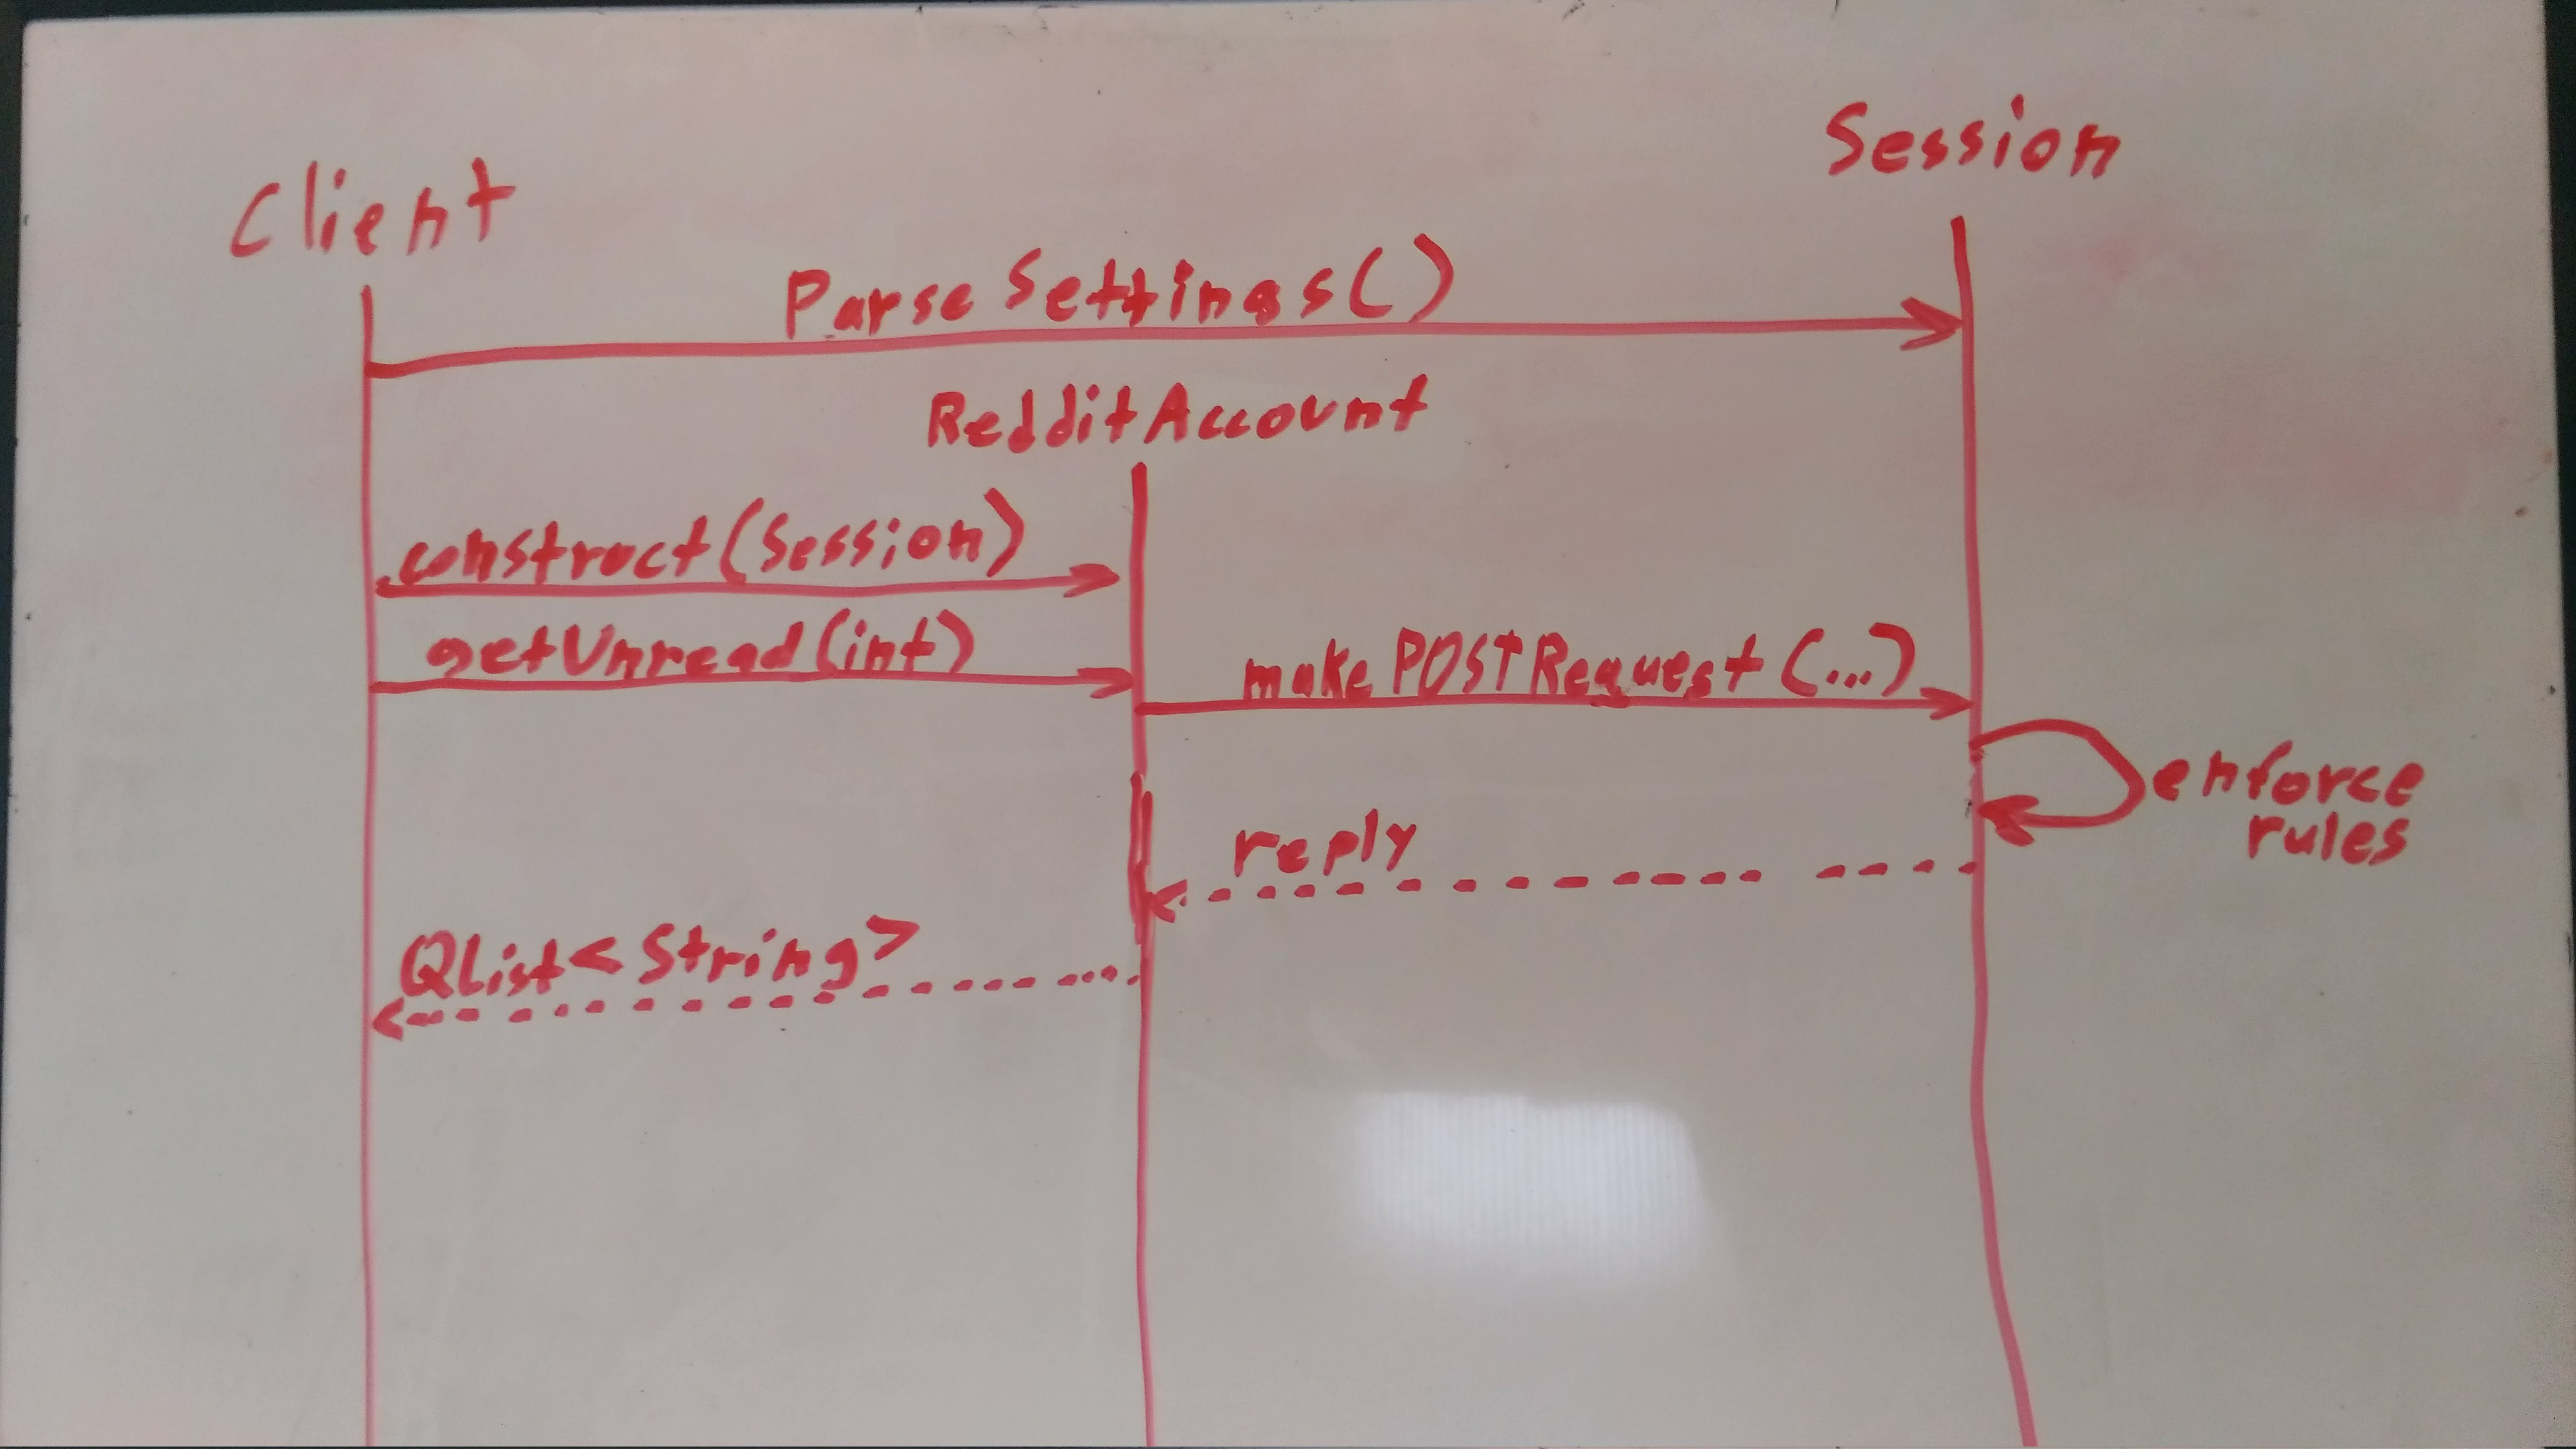
\includegraphics[width=0.65\textwidth]{sequence1.jpg}
	\vspace{-10pt}
\end{figure}
\begin{figure}[ht]
	\centering
	\caption{New Sequence Diagram Example for Getting Data. It has the most interesting example where the comments recursivly parse for new things. Many other calls are just simpler versions of this.}
	\label{sequence2}
	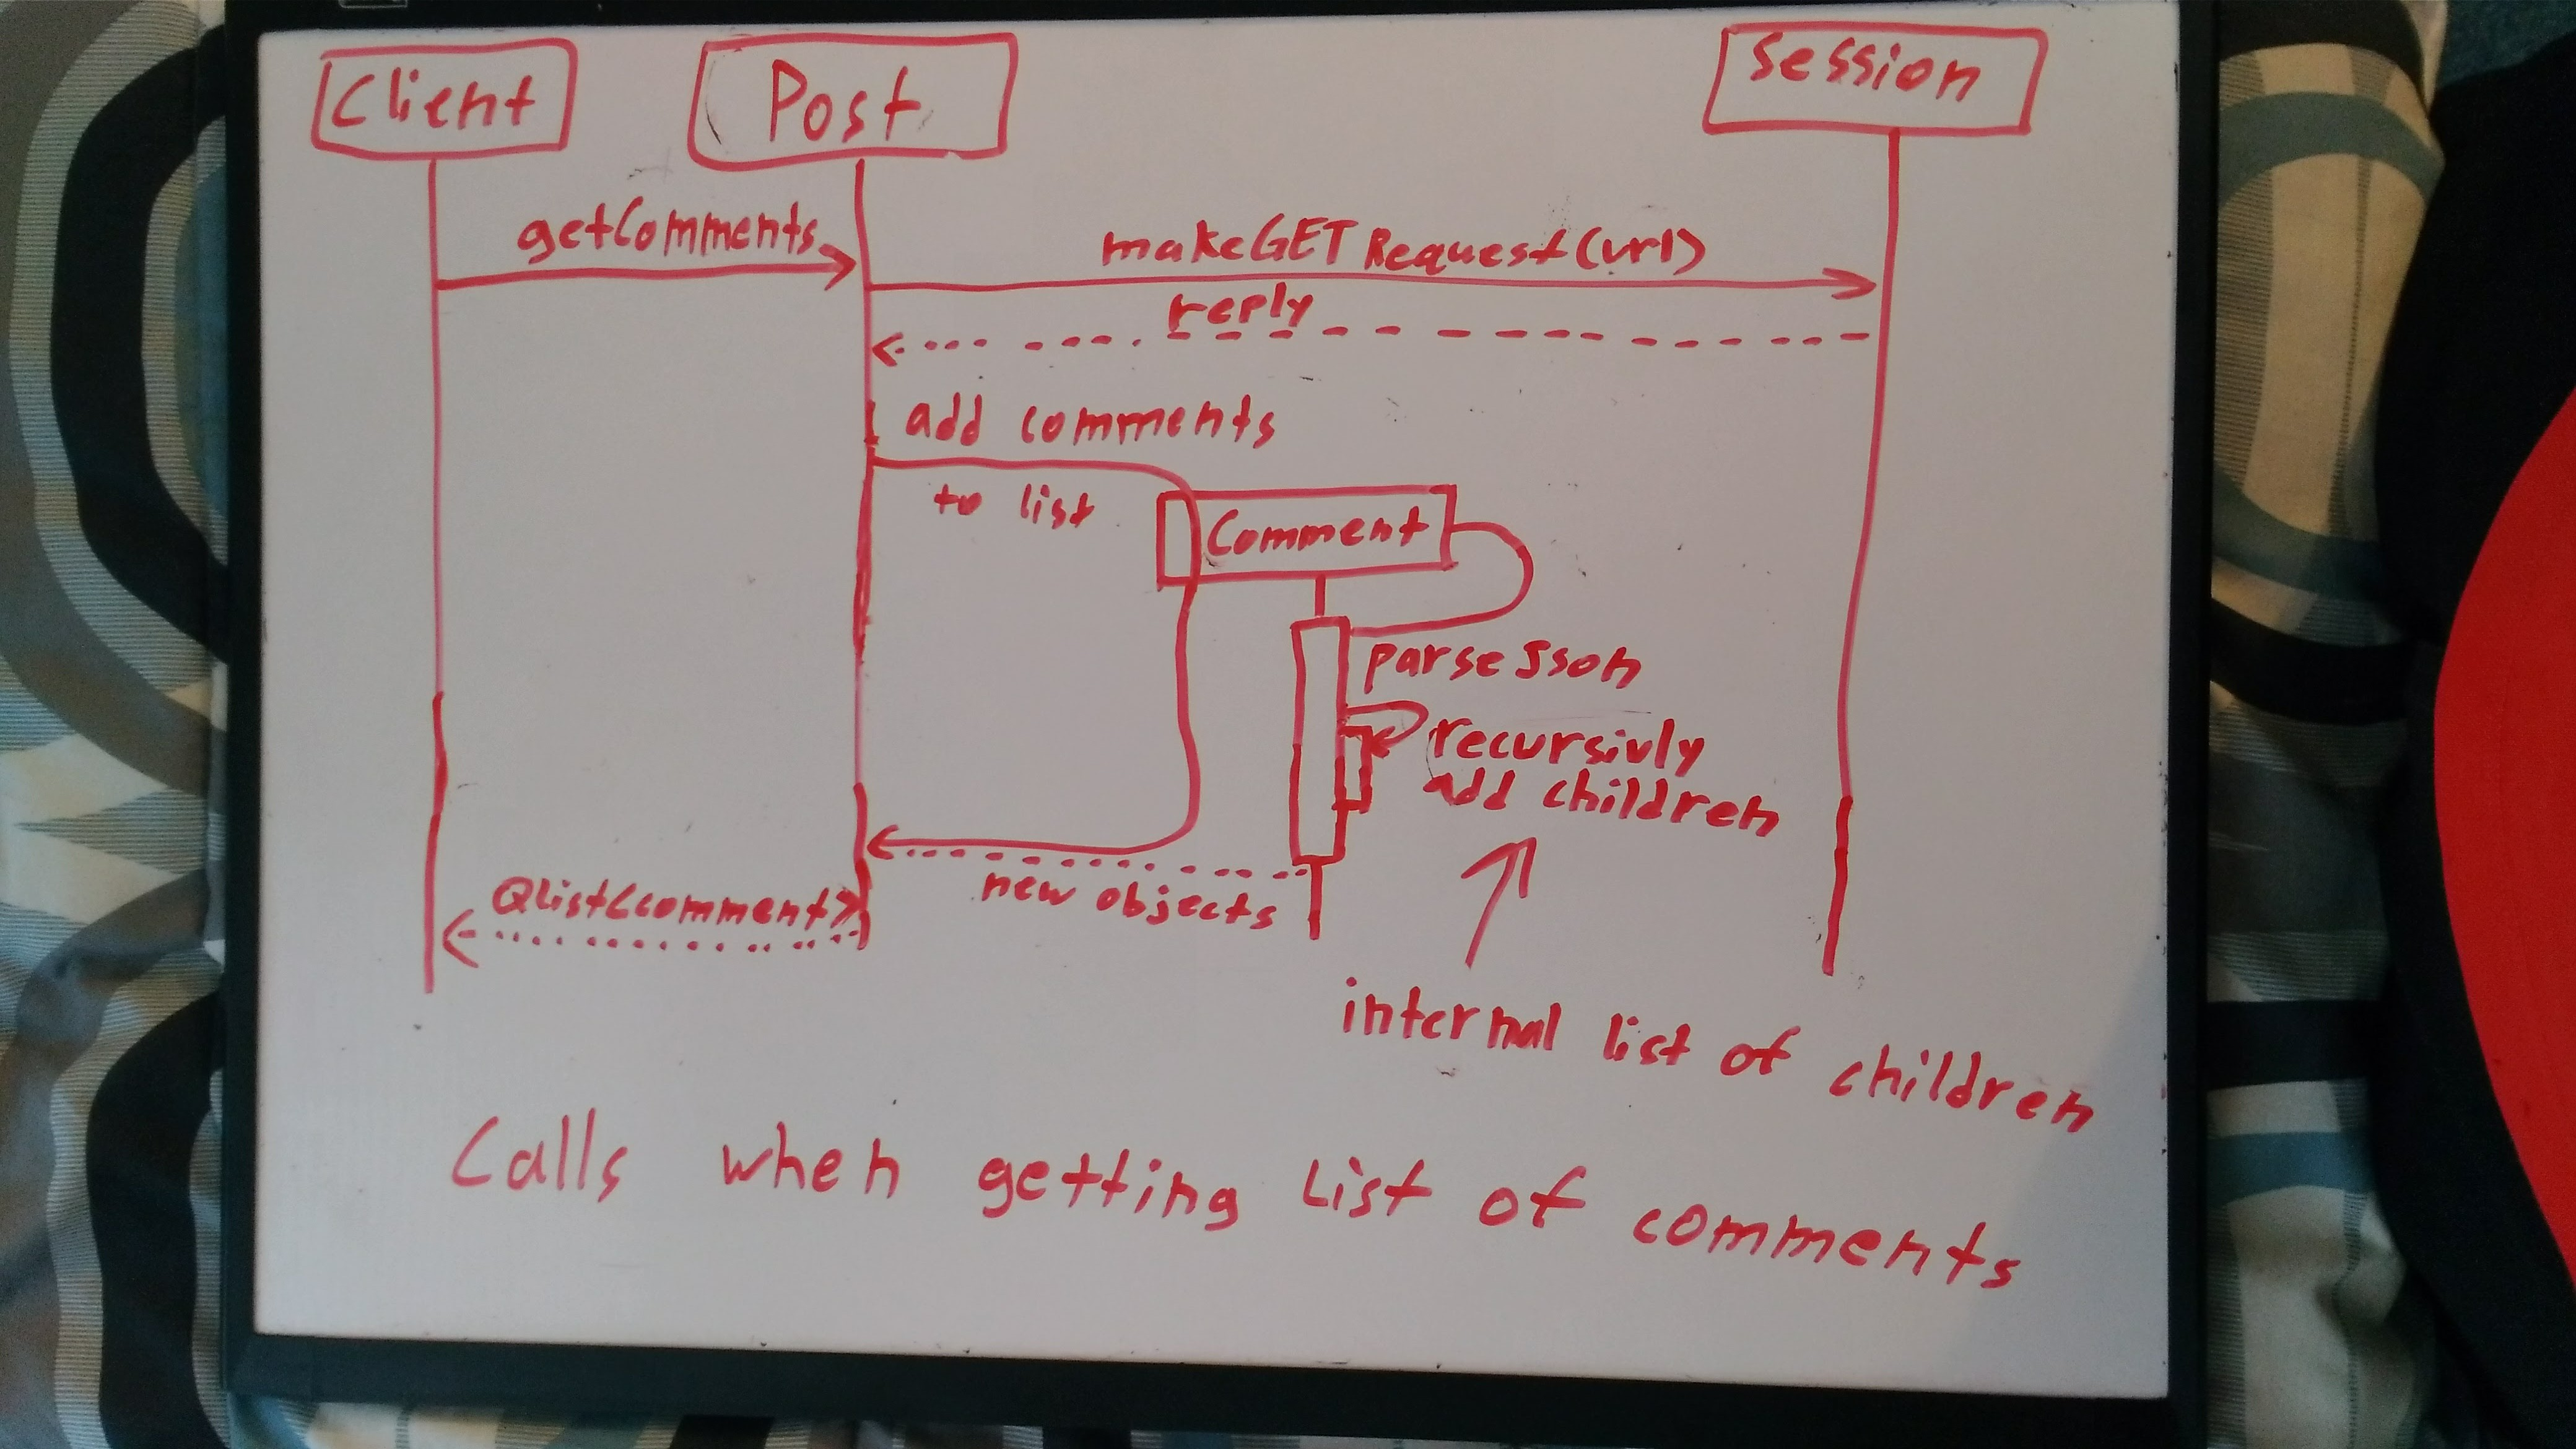
\includegraphics[width=0.65\textwidth]{sequence2.jpg}
	\vspace{-10pt}
\end{figure}

\clearpage
\section{Object Structure}
\begin{figure}[ht]
	\centering
	\caption{Thinking about Object Responsibilities. I made this to just keep my thoughts straight in the middle of coding one day.}
	\label{object_structure2}
	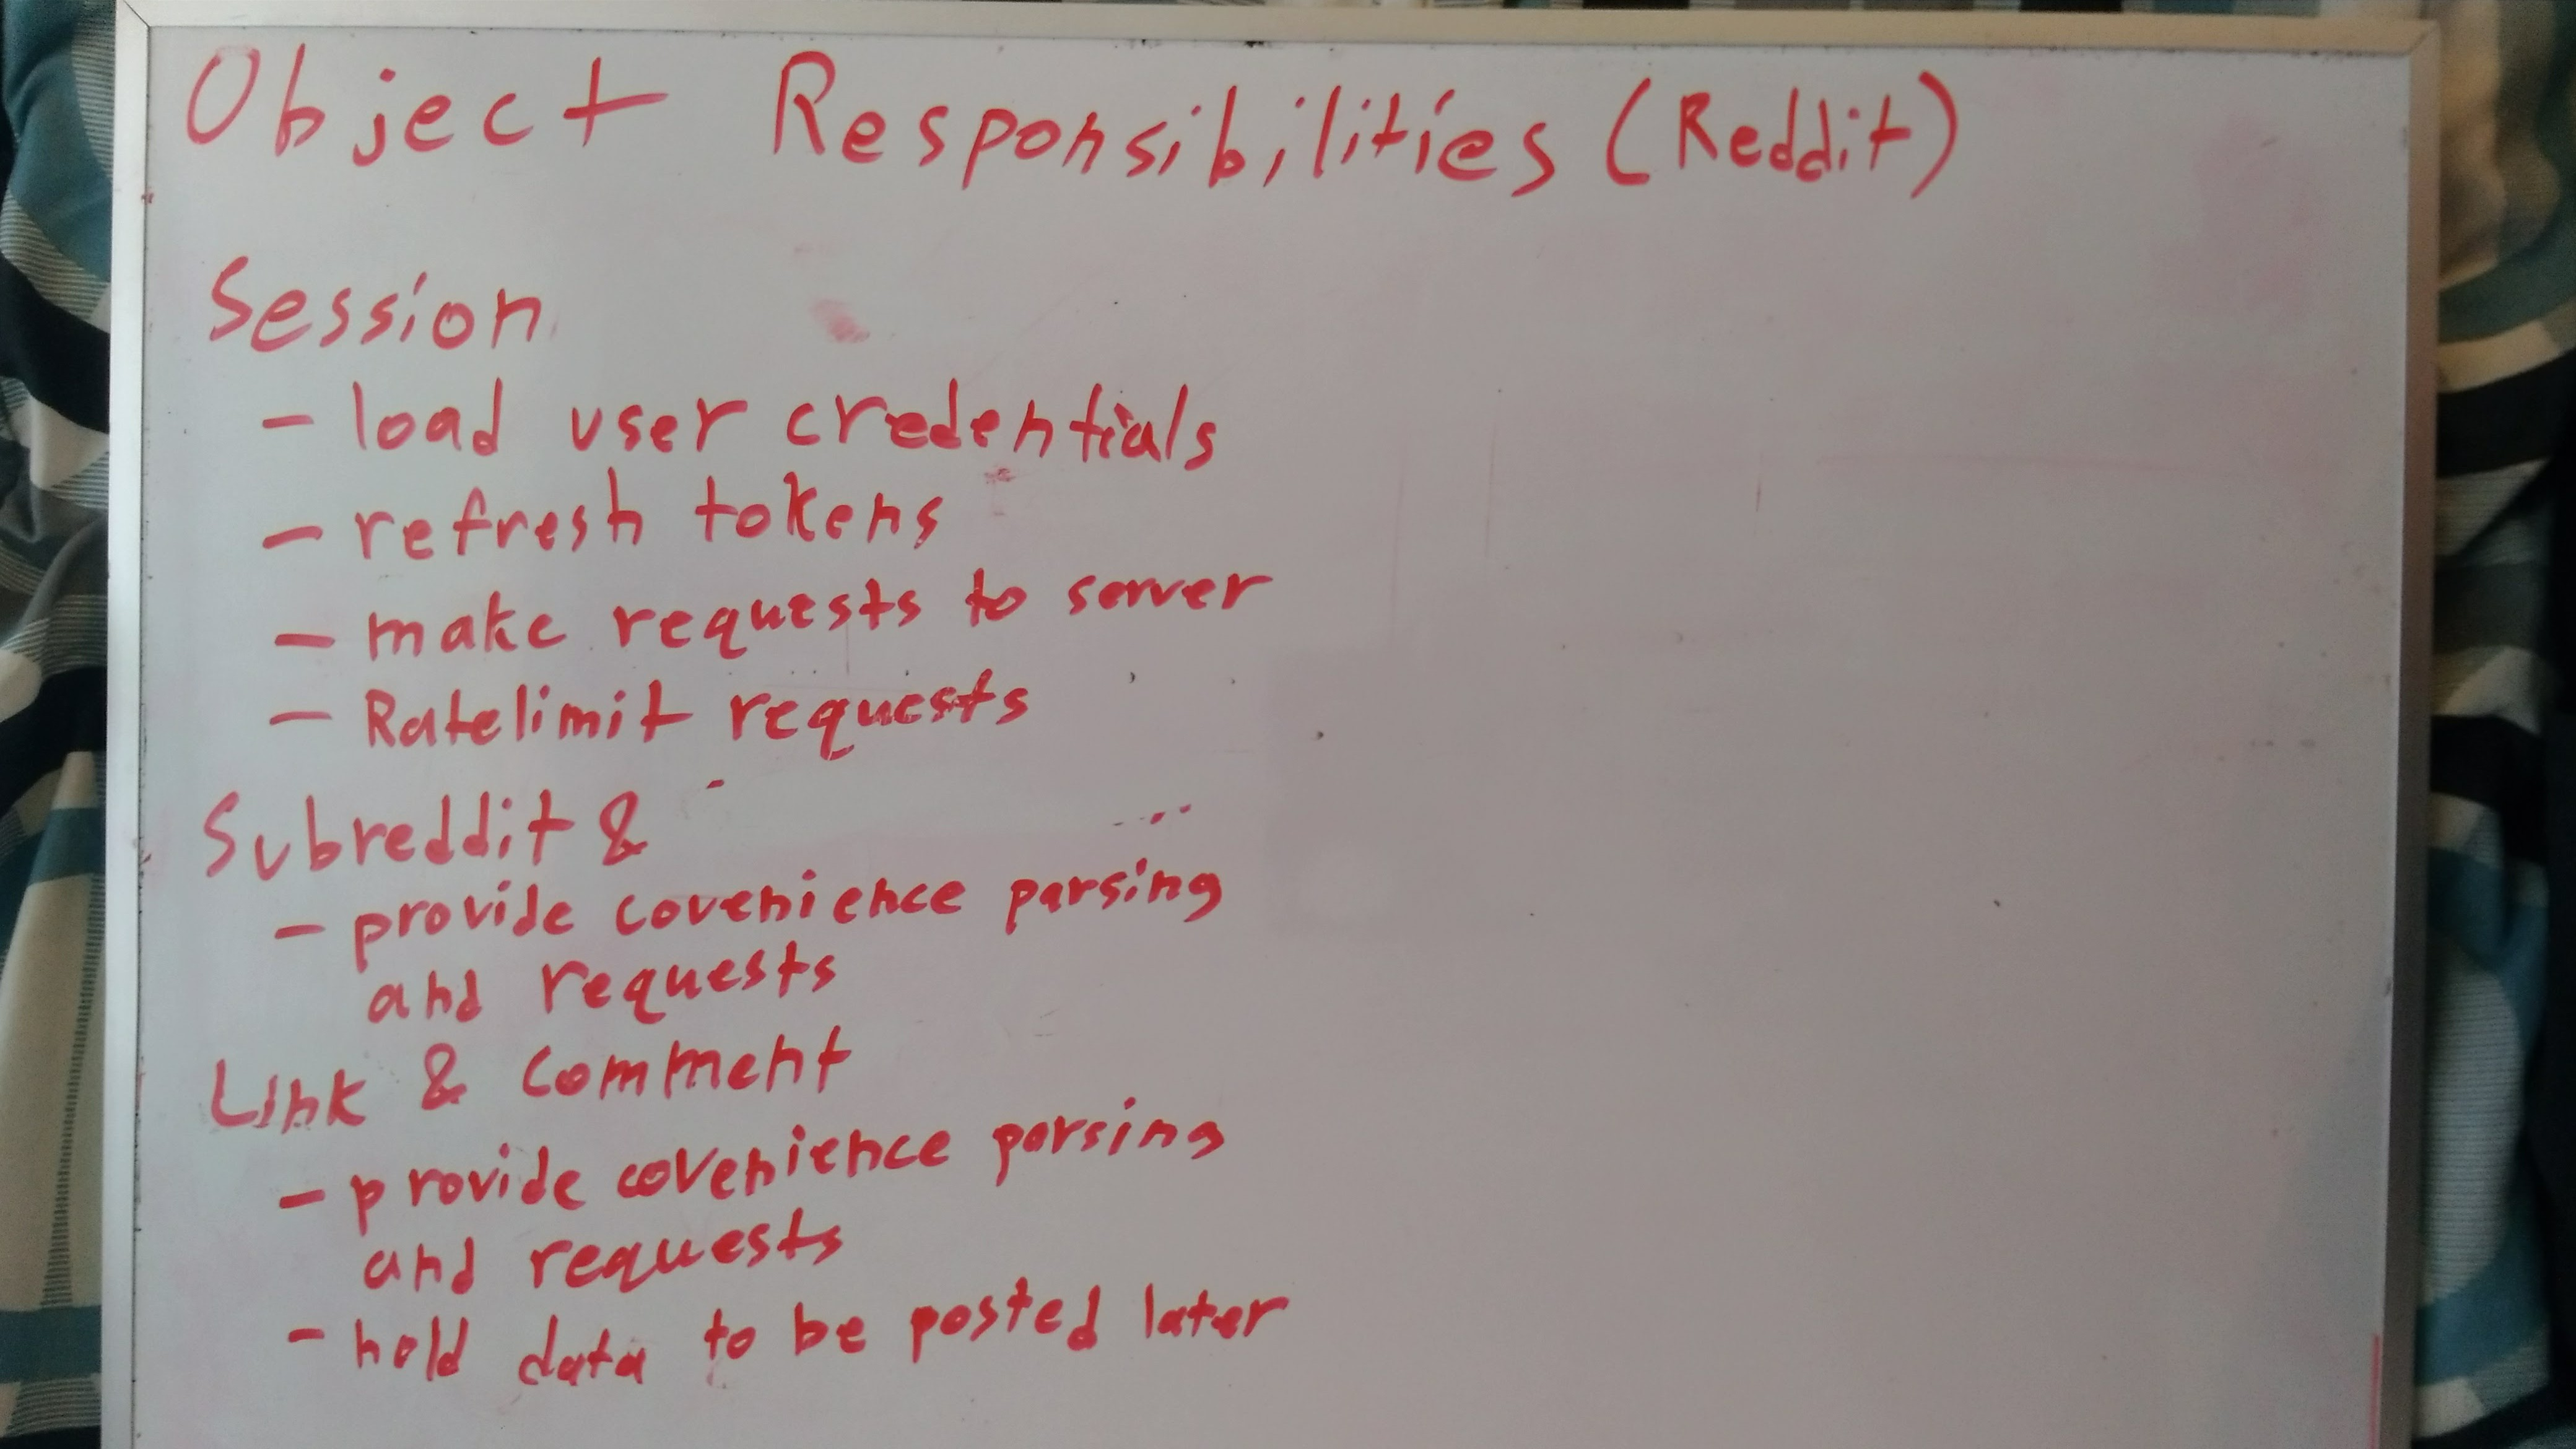
\includegraphics[width=0.65\textwidth]{object_structure2.jpg}
	\vspace{-10pt}
\end{figure}
\begin{figure}[ht]
	\centering
	\caption{Implementing Responsibilities. I made this a little later that day on my second board. It was me thinking about some basics to implement the responsibilities.}
	\label{object_structure1}
	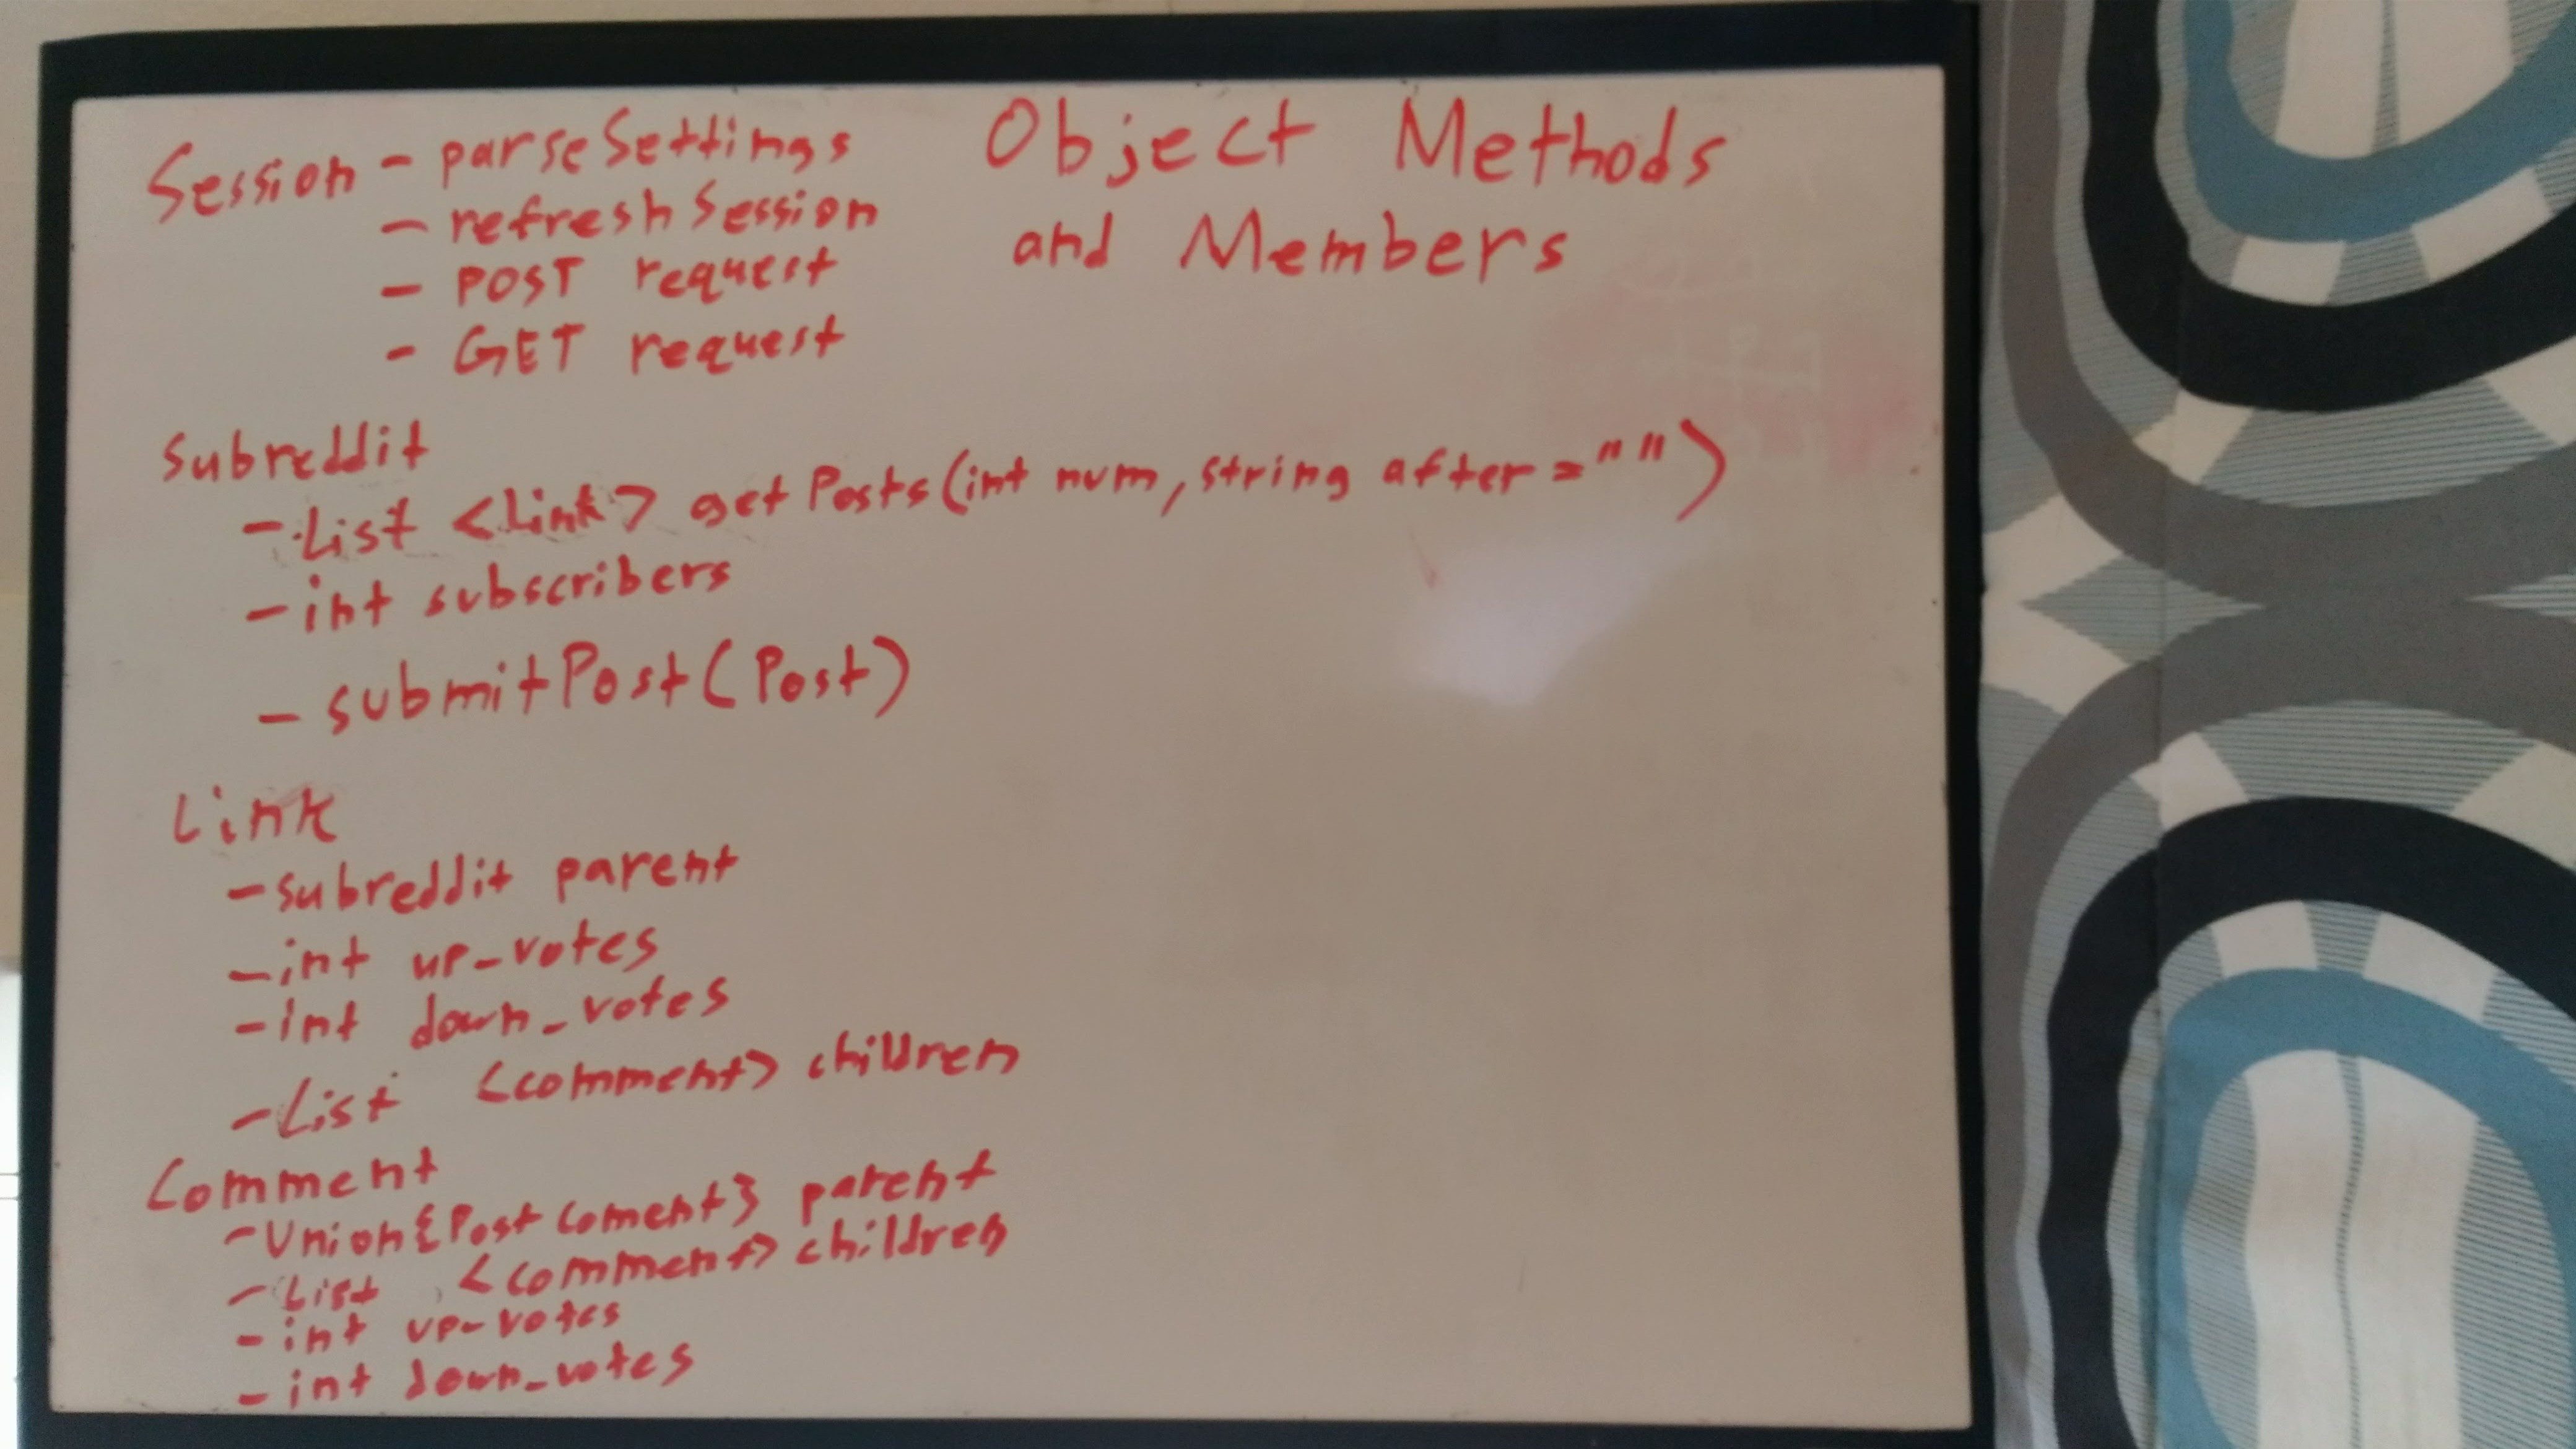
\includegraphics[width=0.65\textwidth]{object_structure1.jpg}
	\vspace{-10pt}
\end{figure}

\clearpage
\section{JSON}
\begin{figure}[ht]
	\centering
	\caption{Original Skectch for JSON Parsing. You can see me using (wrong) notation to show it as a base class of the other objects.}
	\label{json1}
	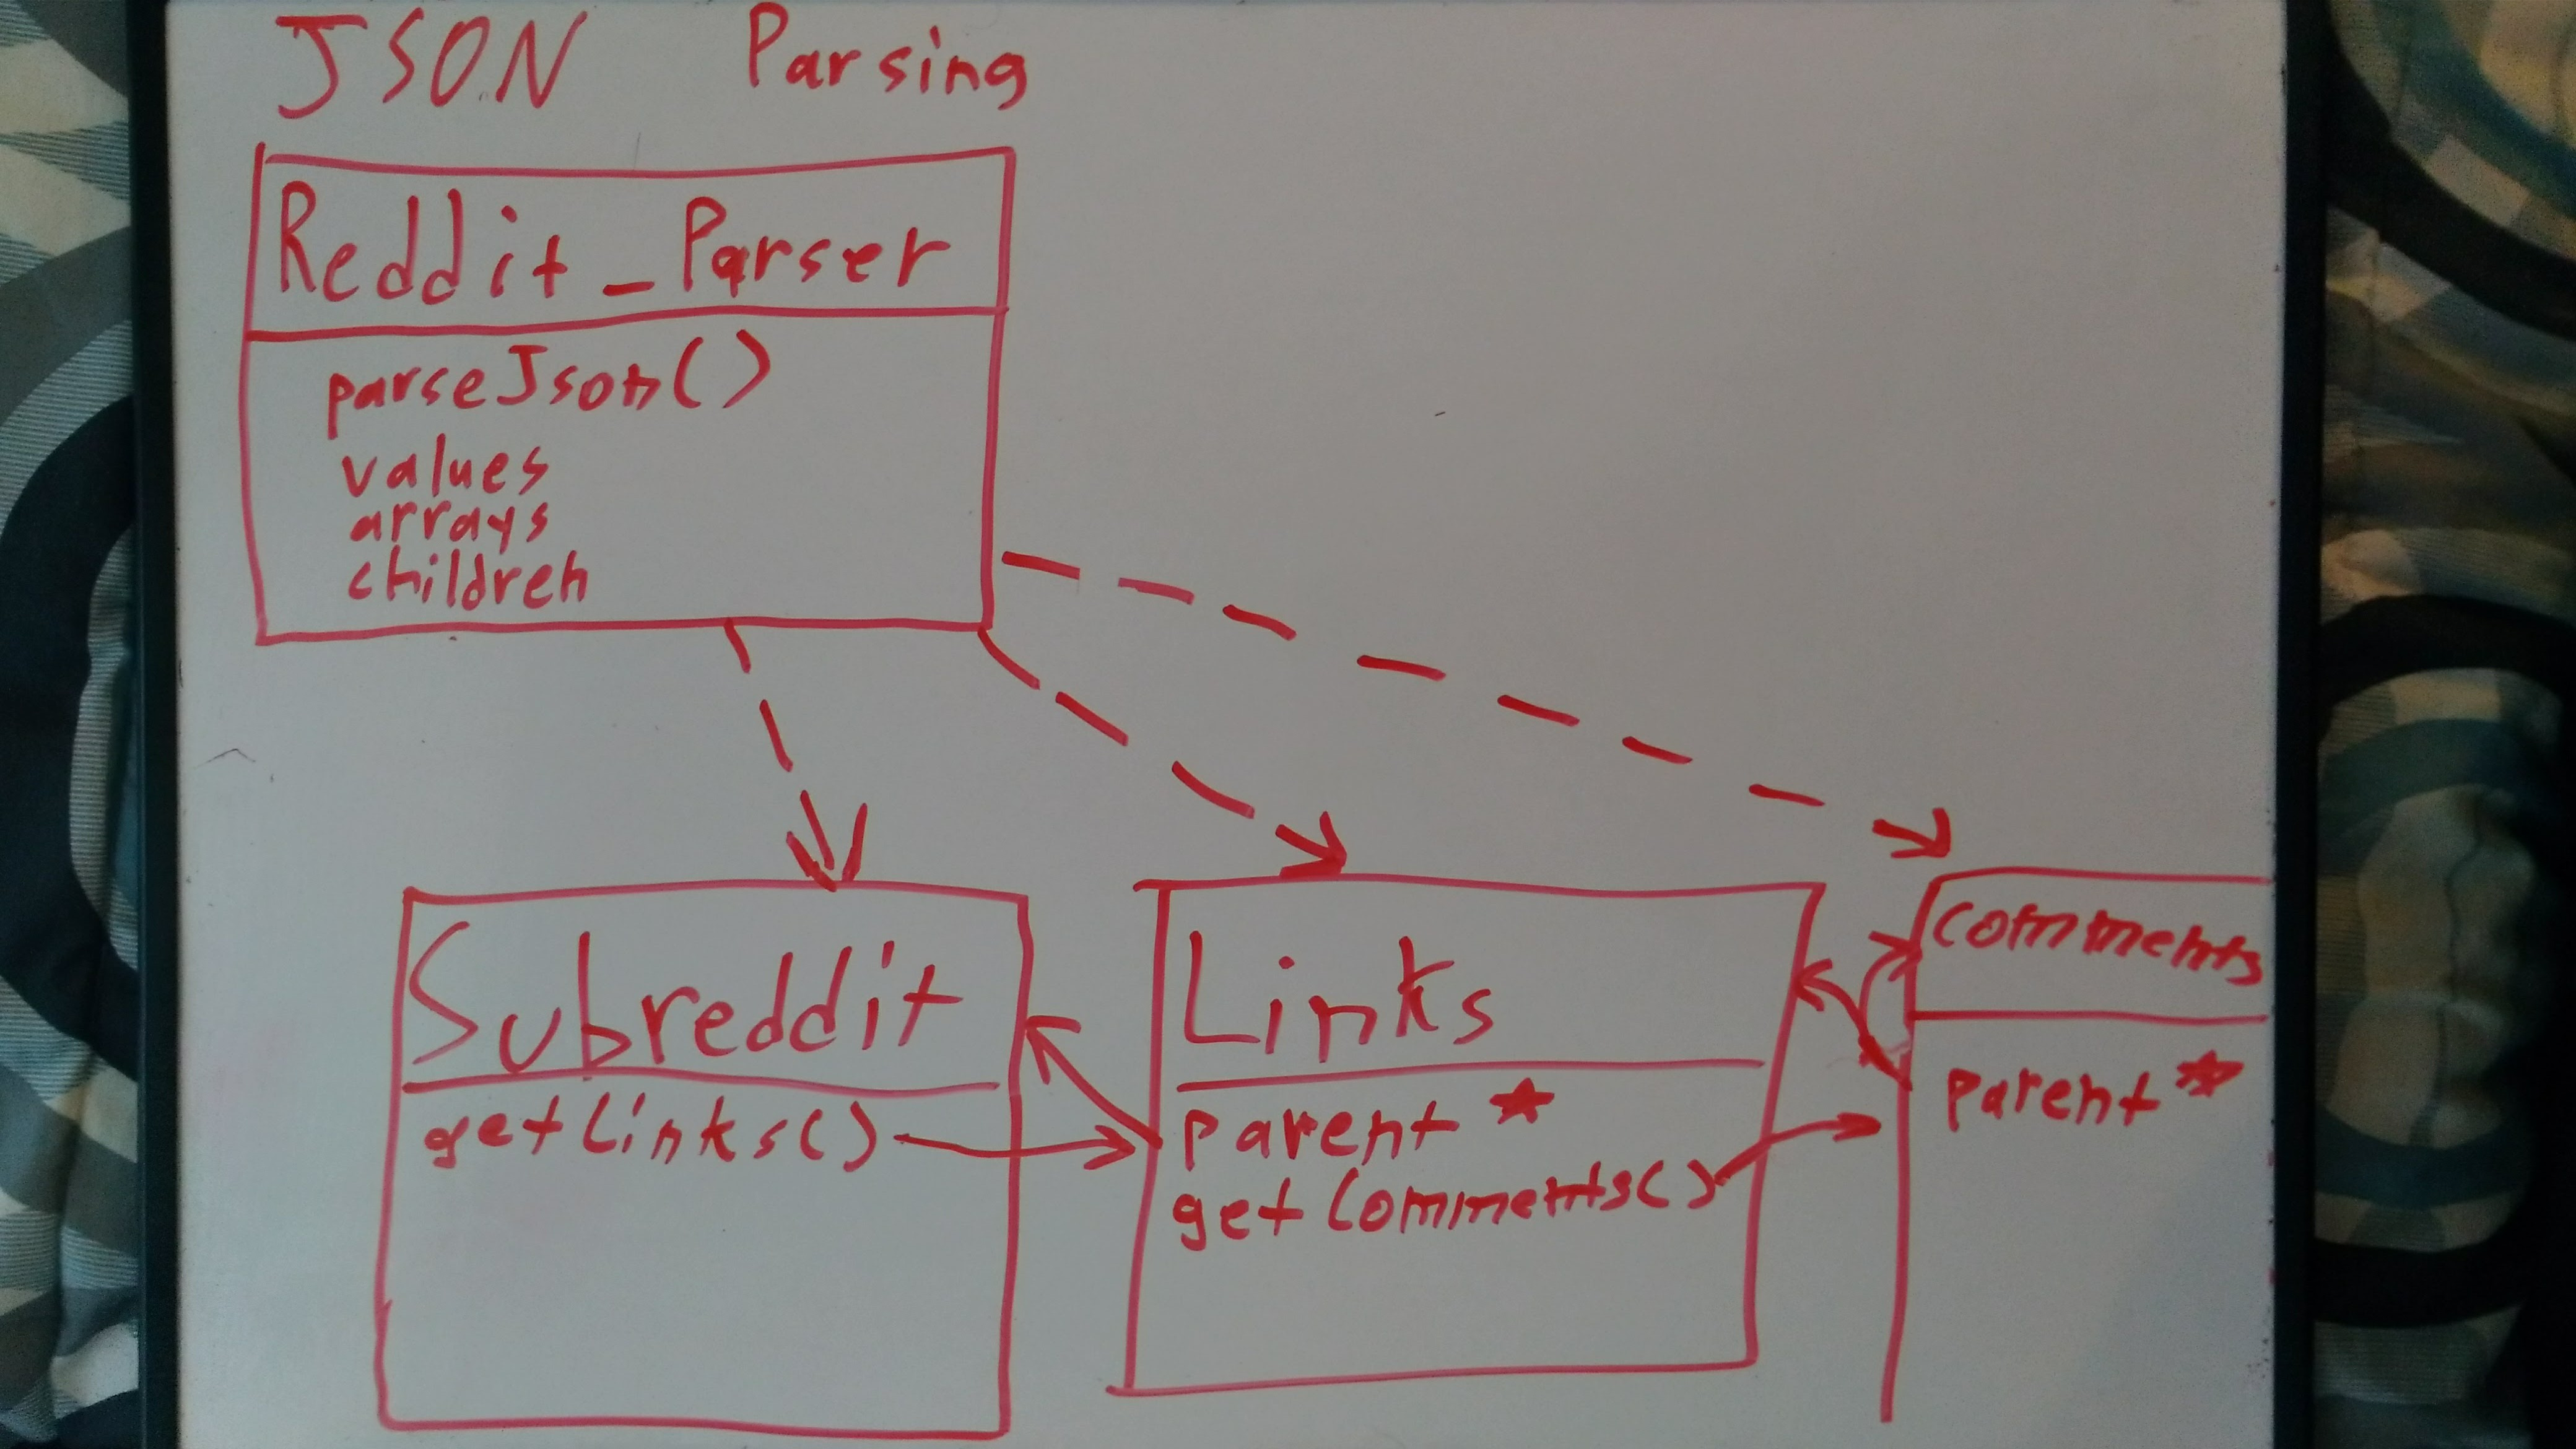
\includegraphics[width=0.65\textwidth]{json1.jpg}
	\vspace{-10pt}
\end{figure}
\begin{figure}[ht]
	\centering
	\caption{JSON Parsing Now. I drew this for this report just as a comparison to the old thing. Objects just do it independently and it is proably less code than if I pre-parsed.}
	\label{json2}
	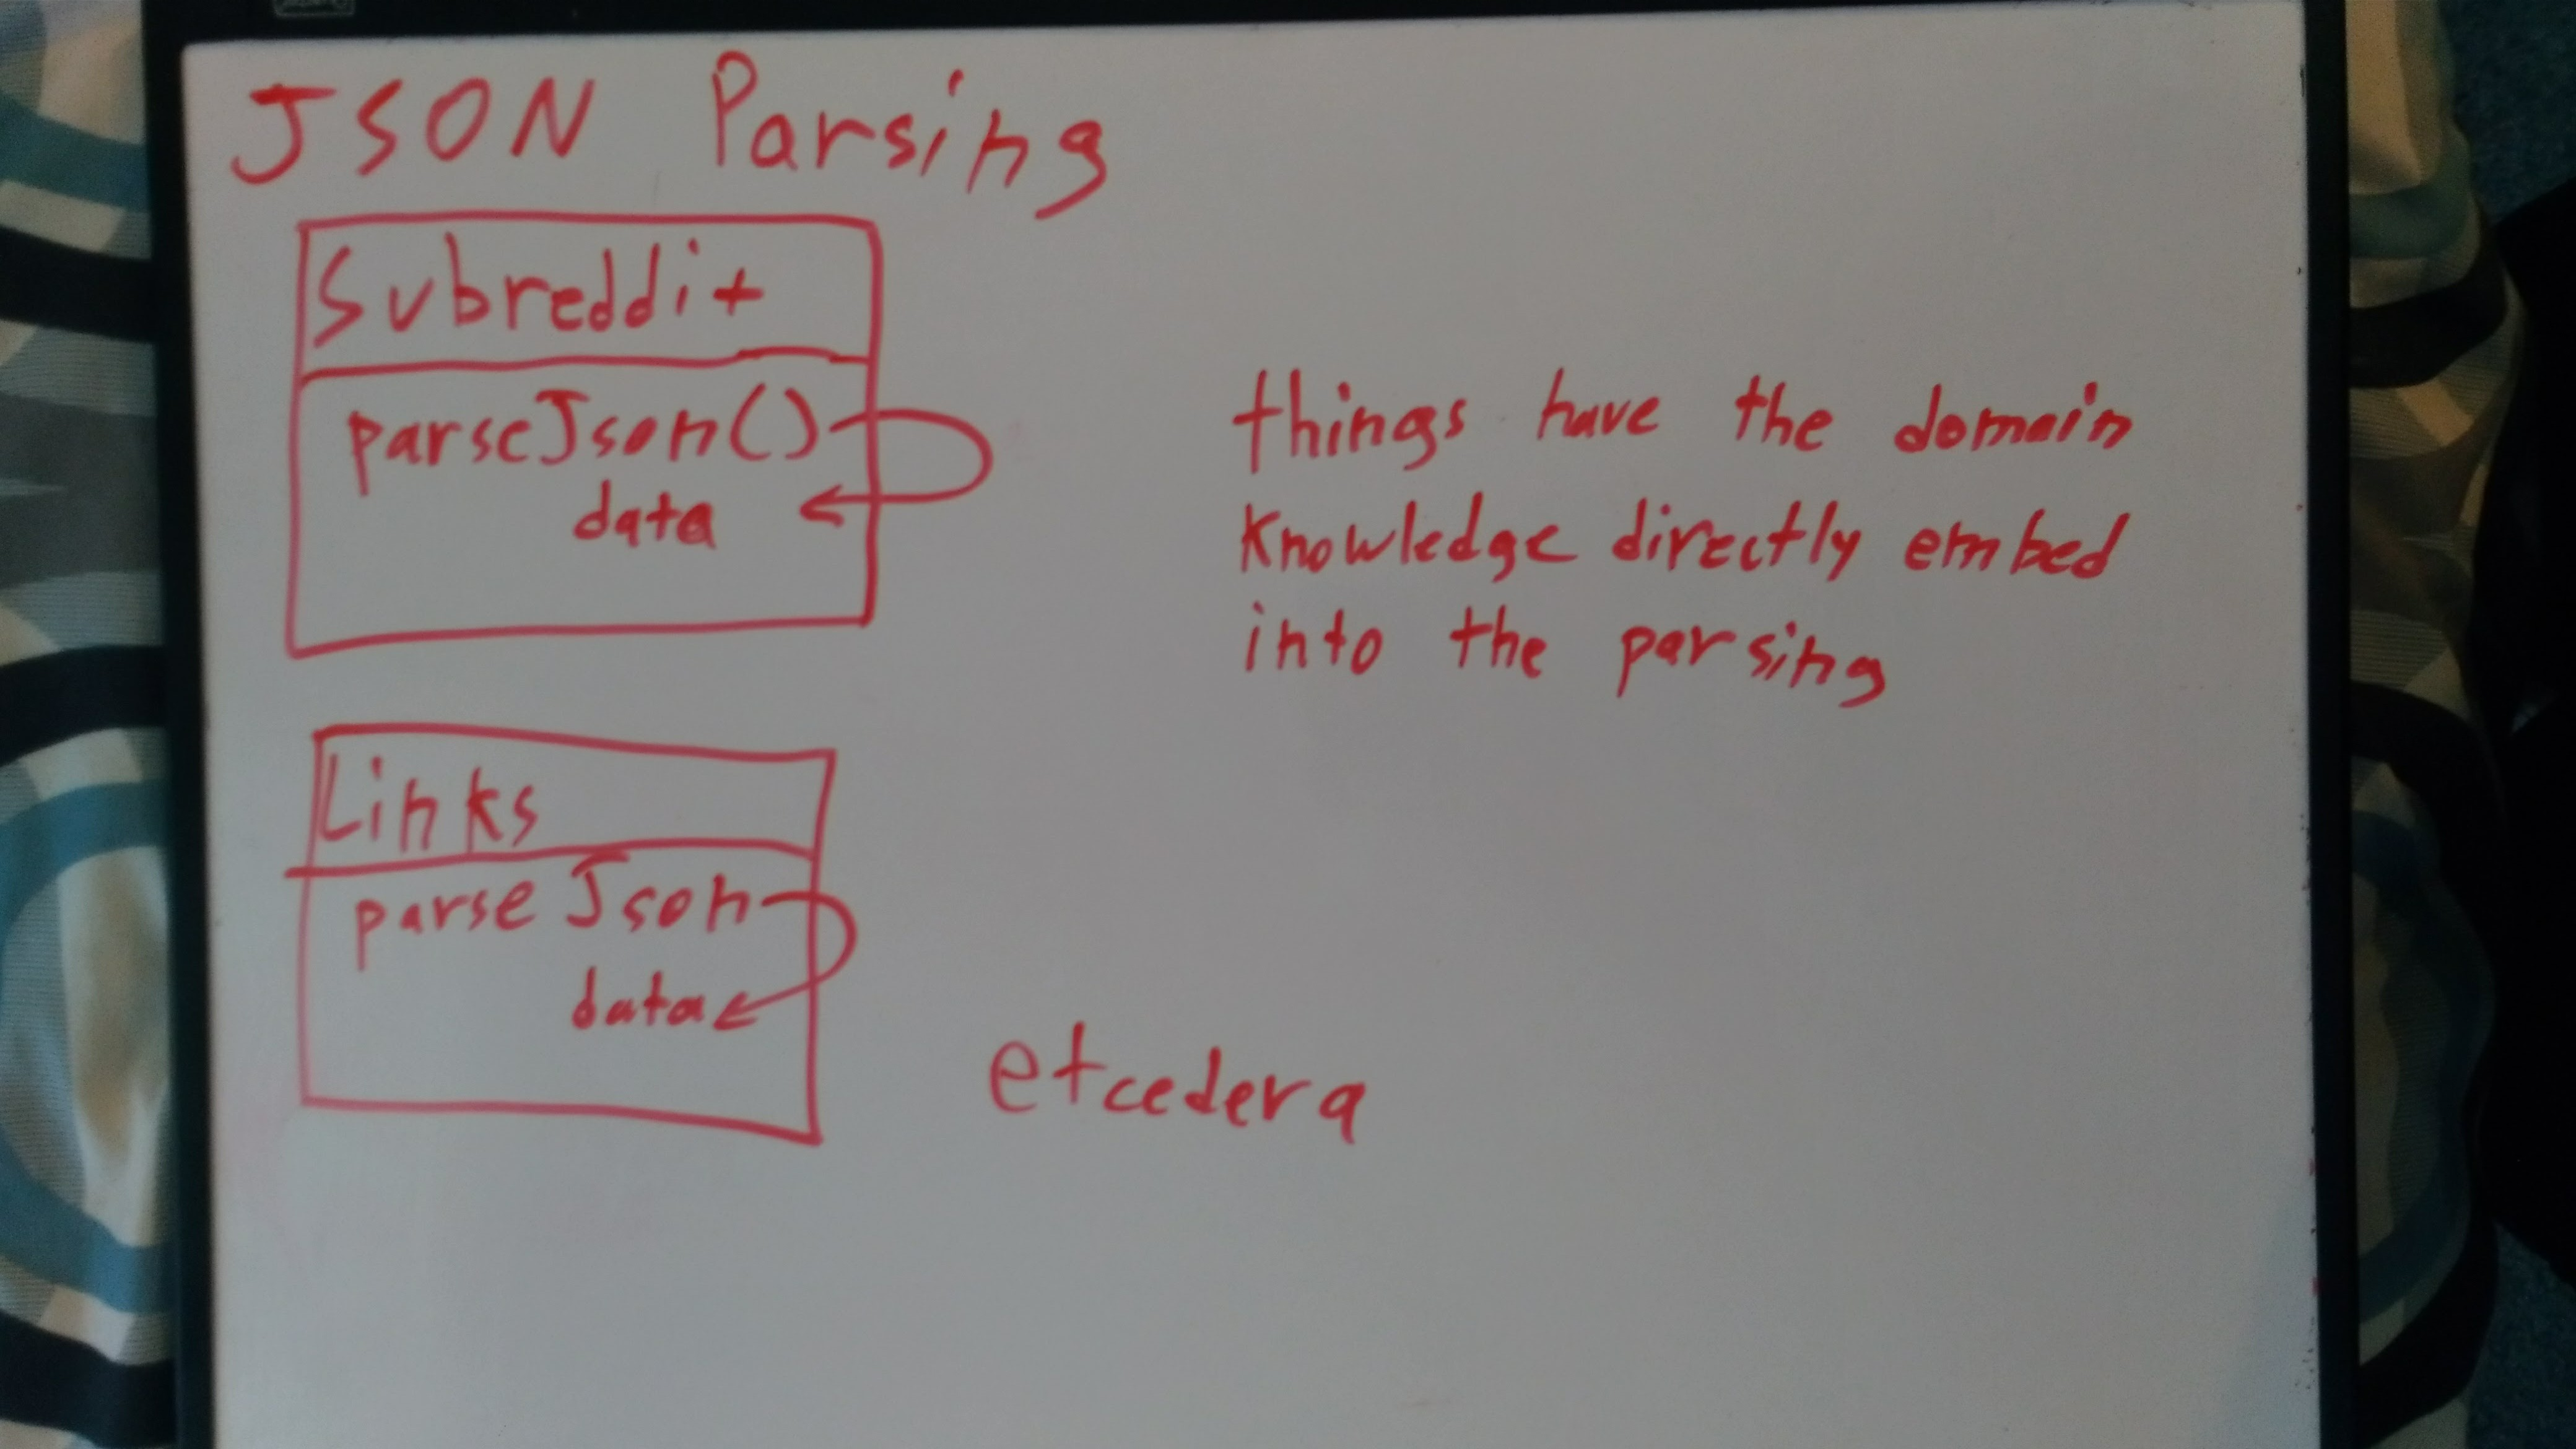
\includegraphics[width=0.65\textwidth]{json2.jpg}
	\vspace{-10pt}
\end{figure}

\clearpage
\section{Client Example Code}
\begin{figure}[ht]
	\centering
	\caption{Idealized API Code Usage. I like to do this sometimes for different things. It makes me do a sanity check for what I want the API of the objects I'm making to be. I guess this is ensuring proper responsibilities if I were to talk in terms of the book, but historically I just felt that things were weird if I meander through coding.}
	\label{json1}
	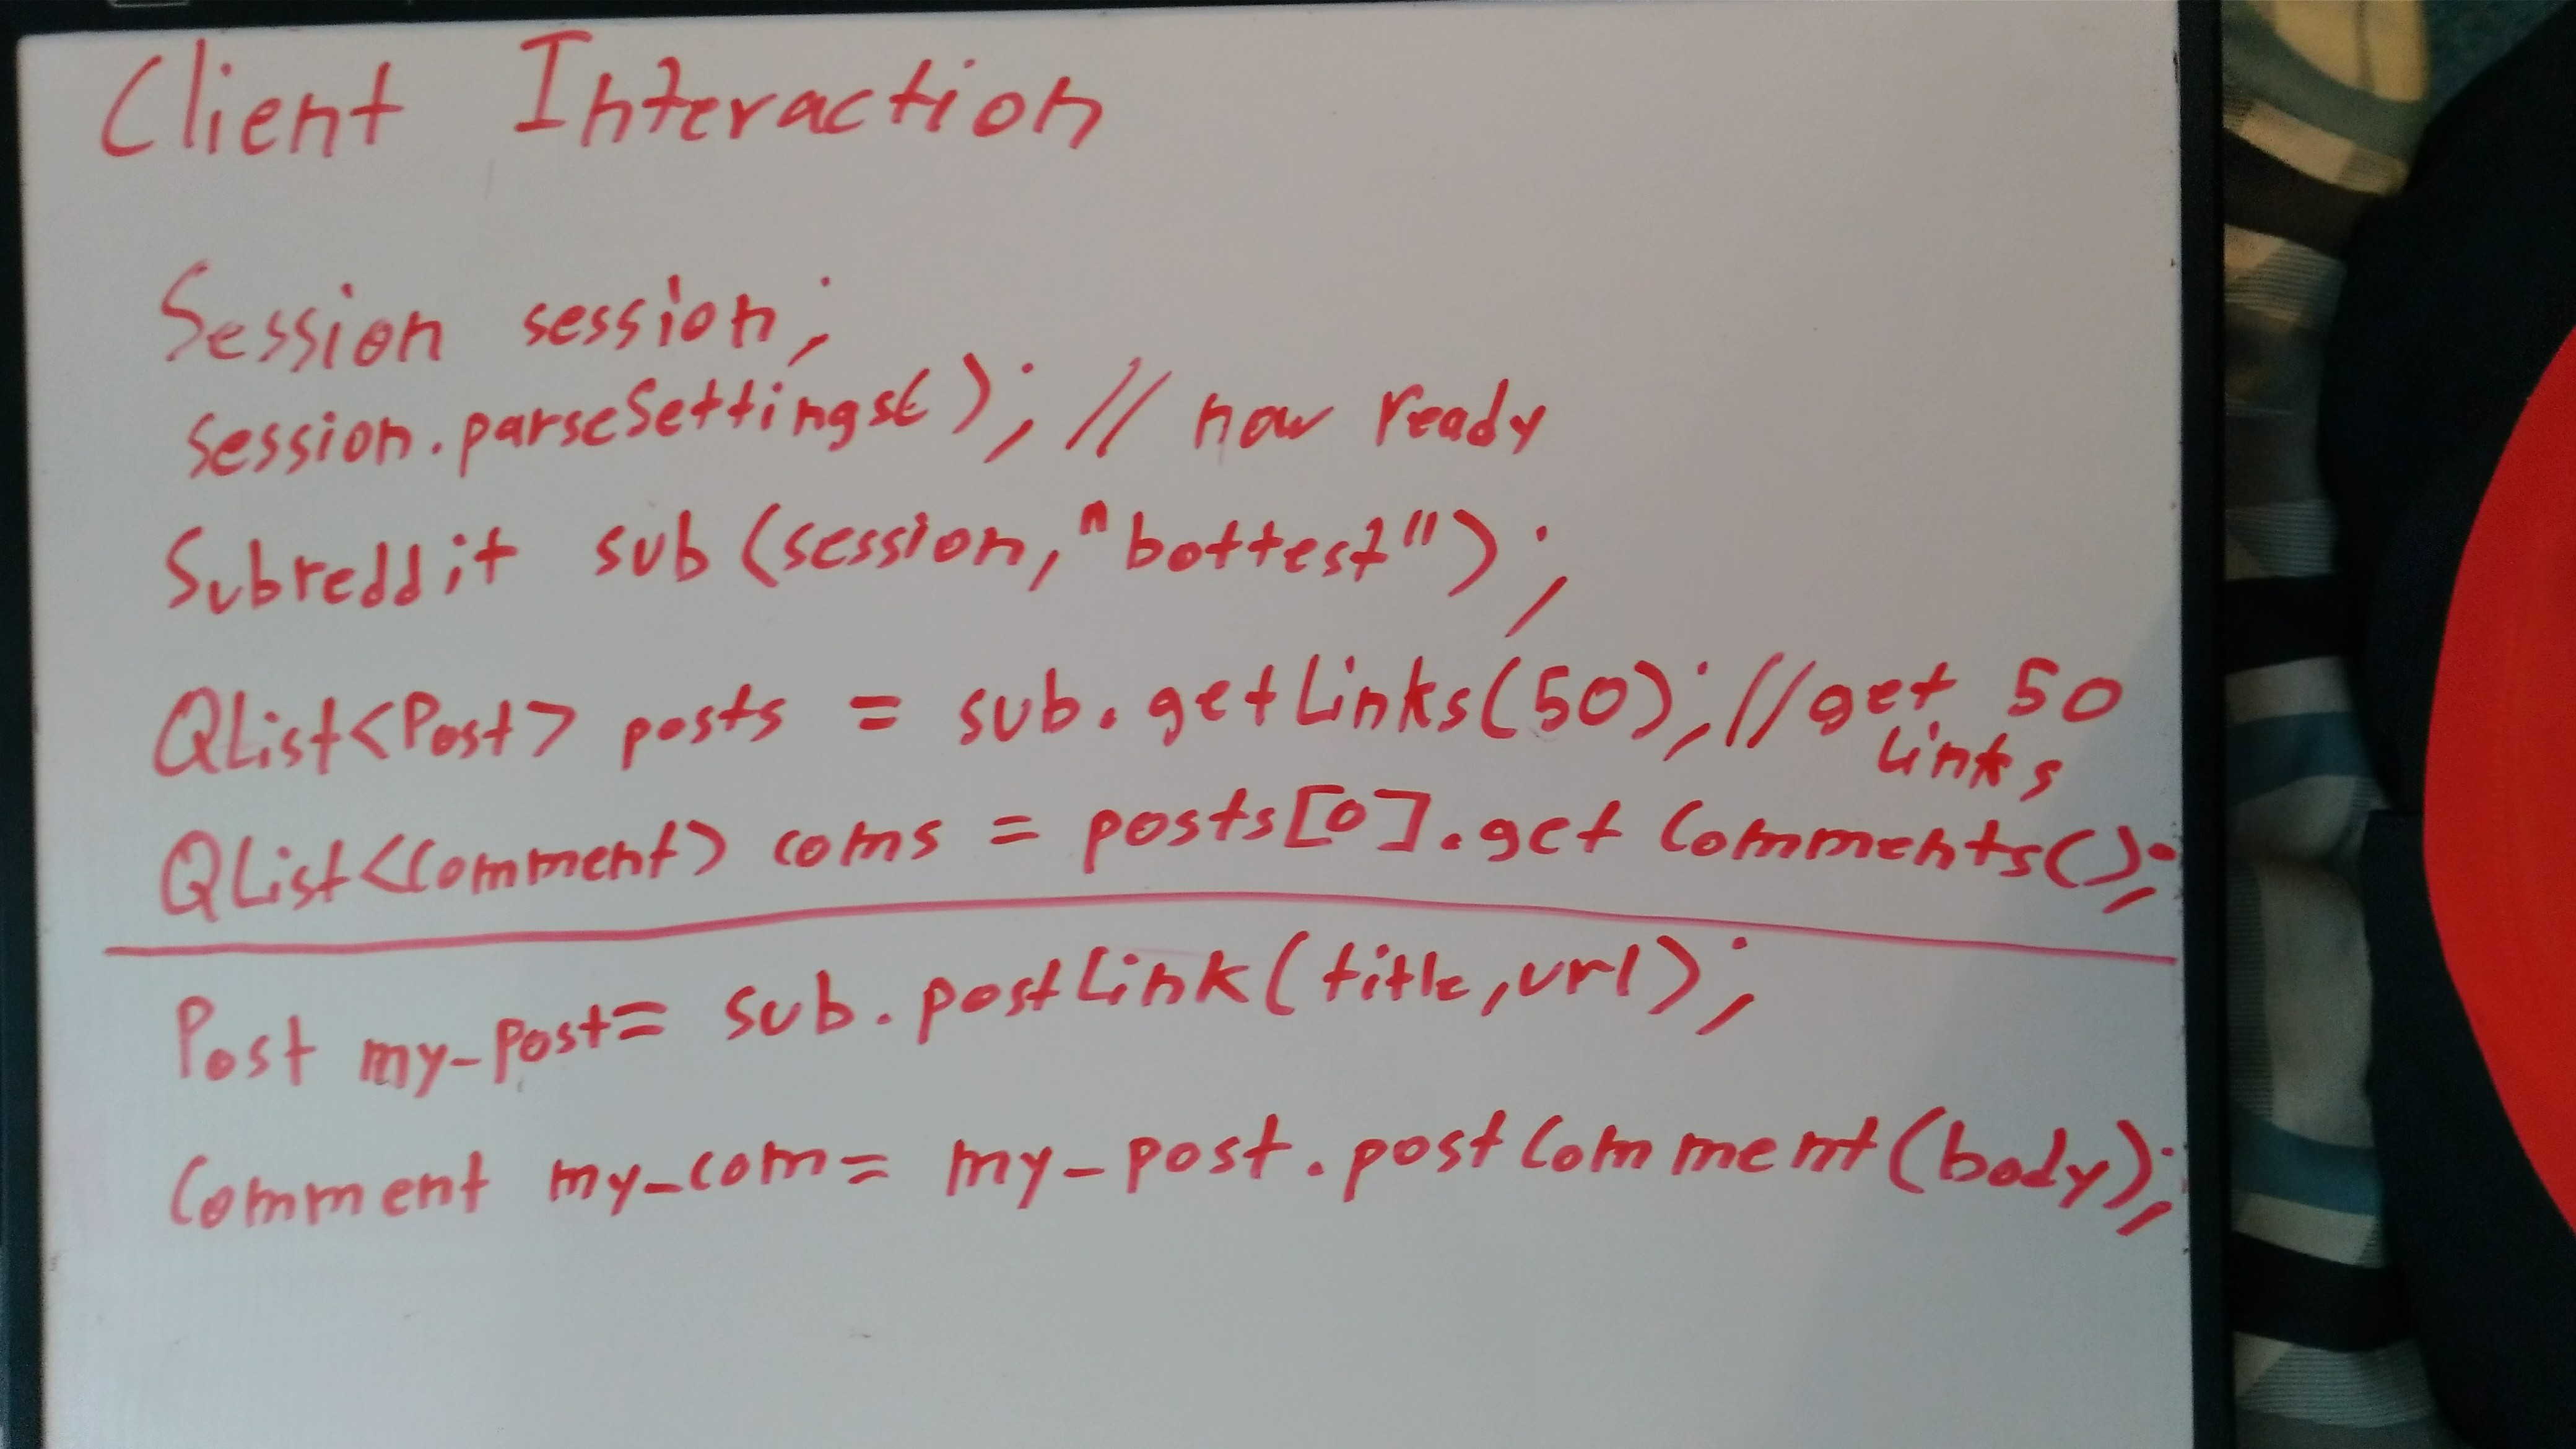
\includegraphics[width=0.65\textwidth]{client_example_code.jpg}
	\vspace{-10pt}
\end{figure}

\end{document}